\documentclass[12pt,a4paper]{article}
\usepackage[top=75pt, bottom=75pt, left=75pt, right=75pt]{geometry}
\usepackage[utf8]{inputenc}
\usepackage[T1]{fontenc}
\usepackage{natbib}
\usepackage[spanish]{babel}
\bibliographystyle{alpha}
\usepackage[hyperfootnotes=true,colorlinks=true]{hyperref}
\newcommand\fnurl[2]{\href{#2}{#1}\footnote{\url{#2}}}
\newcommand\mono[1]{\texttt{#1}}
\usepackage{color}
\usepackage{listings}
\usepackage{bold-extra}
\usepackage{amsfonts}
\usepackage{caratula}
\lstset
{
	language=[Sharp]C,              % choose the language of the code
	basicstyle=\ttfamily,           % the size of the fonts that are used for the code
	keywordstyle=\ttfamily\color[rgb]{0,0.5,1},
	numbers=left,                   % where to put the line-numbers
	numberstyle=\scriptsize,        % the size of the fonts that are used for the line-numbers
	stepnumber=1,                   % the step between two line-numbers. If it is 1 each line will be numbered
	numbersep=10pt,                 % how far the line-numbers are from the code
	backgroundcolor=\color{white},  % choose the background color. You must add \usepackage{color}
	showspaces=false,               % show spaces adding particular underscores
	showstringspaces=false,         % underline spaces within strings
	showtabs=false,                 % show tabs within strings adding particular underscores
	frame=lines,                    % adds a frame around the code
	tabsize=2,                      % sets default tabsize to 2 spaces
	captionpos=b,                   % sets the caption-position to bottom
	breaklines=true,                % sets automatic line breaking
	breakatwhitespace=false,        % sets if automatic breaks should only happen at whitespace
	escapeinside={\%}{)}            % if you want to add a comment within your code
}
\lstset{emph={Contract,Memory,Rsd,Tmp,DestRsd,DestTmp,BindRsd,This,Return,AddRsd,AddTmp,IterationSpace,RsdType,System,Diagnostics,Contracts,Requires,Ensures,Assume,Assert,Result},emphstyle=\color[rgb]{1,0.6,0}}
\renewcommand\lstlistingname{Ejemplo}
\renewcommand\lstlistlistingname{Ejemplos} %para \lstlistoflistings
\def\lstlistingautorefname{Ejemplo} %para \autoref{label}

\begin{document}

	\materia{Tesis de Licenciatura}

	\titulo{Especificación y verificación modular de consumo de memoria}

	\integrante{Jonathan Tapicer}{371/06}{jtapicer@dc.uba.ar}

	\director{Diego Garbervetsky}{diegog@dc.uba.ar}
	\director{}{}
	\director{}{}
	\director{}{}
	\director{}{}
	\director{Martín Rouaux}{mrouaux@dc.uba.ar}

	\fecha{Febrero de 2011}

	\maketitle

	\newpage

	\setlength{\parskip}{4pt}
	\linespread{1.3}

	\vspace*{-15pt}
	\begin{abstract}
		% problema, inferencia, proponemos verificación
		Abordamos en este trabajo la problemática de la verificación modular del consumo de memoria en programas orientados a objetos. El enfoque propuesto consiste en permitir al usuario anotar el programa con contratos asociados al consumo de memoria del mismo y luego verificar su correctitud, obteniendo así un \textit{certificado} del consumo máximo de memoria del programa.
		\\
		
		%para modelo de mem por reg, definimos un lenguaje (sintaxis y semantica) para contratos modulares intuituivo, expresivo (tiempo de vida) oculta info
		Para representar el hecho de que la memoria es recolectada automáticamente por un \textit{garbage collector} en los lenguajes orientados a objetos del estilo de Java y C\#, utilizaremos un modelo simplificado de administración de memoria basado en scopes. Definimos la sintaxis y semántica de un lenguaje de anotaciones para escribir contratos modulares de consumo de memoria en el código. Este lenguaje es suficientemente expresivo para brindar información de tiempo de vida de los objetos y contempla mecanismos de ocultamiento de la información para mantener la modularidad.
		\\
		
		%definimos técnicas de instrumentación y verificación, apoyandose en verif existente
		Se diseñan y detallan un conjunto de técnicas de instrumentación y verificación de los contratos, que apoyadas en un verificador estático permiten desarrollar una solución capaz de verificar la correctitud de los contratos dados en las anotaciones definidas.
		\\
		
		%integración de herramientas externas para mejorar la aritmética
		La verificación de los contratos requiere muchas veces de una capacidad de análisis aritmético complejo. Dadas las limitaciones en el módulo aritmético de las mayoría de los verificadores estáticos existentes, proponemos un conjunto de técnicas adicionales que permiten integrar herramientas externas al proceso de verificación, haciendo posible la verificación de contratos con requerimientos aritméticos complejos.
		\\
		
		%implementación de prueba de concepto para .net y code contracts
		Realizamos una implementación de prueba de concepto de las anotaciones y técnicas desarrolladas en el trabajo para la plataforma .NET utilizando las capacidades de verificación de la herramienta Code Contracts.
	\end{abstract}

	\linespread{1}

	\newpage
	\tableofcontents

	\newpage
	\lstlistoflistings
	\listoffigures

	\newpage
	\setlength{\parskip}{\baselineskip}
	\section{Introducción}
		\subsection{Descripción de la problemática}
			En determinado conjunto de aplicaciones la memoria es un recurso crítico para el correcto funcionamiento del sistema; nos referimos a sistemas donde el uso de memoria debe ser predecible y determinístico tales como:

			\begin{itemize}
				\item Aplicaciones para sistemas embebidos, donde muchas veces por limitantes de hardware la memoria suele ser uno de los recursos más importantes a tener en cuenta.
				\item Sistemas real-time, donde no son afrontables los recursos consumidos por un garbage collector y su impredecibilidad temporal\footnote{Es decir, no se puede determinar el momento en el que el \textit{garbage collector} se ejecutará, y esto podría generar un retraso no afrontable por un sistema en tiempo real.}.
				\item Sistemas que se ejecutan en entornos donde el uso de los recursos, y en particuar el uso de memoria, se cobra; en estos casos no es deseable pagar por el uso una cantidad de memoria que no se necesite.
			\end{itemize}

			En estos casos es valioso contar con un \textit{certificado} de que el consumo de memoria del programa nunca excederá un límite dado.

			Un ejemplo de un conjunto de herramientas diseñadas para este fin surge a partir de un movimiento llamado Real-time Java que cuenta con una especificación formal definida en \cite{RTSJ} (Real-time Specification for Java); esta especificación permite implementar Java para sistemas en tiempo real y embebidos con una administración de memoria con consumo predecible (se encuentra disponible una implementación hecha por Sun: \cite{implSun}).

			Es en este marco donde surgen diferentes formas de administración de la memoria dinámica. La administración de memoria por scopes es una de ellas, de la que hablamos en la sección siguiente.

			Un enfoque posible para obtener un \textit{certificado} de consumo de memoria es el tomado por trabajos anteriores como \cite{Rou09}. Este consiste en utilizar técnicas de análisis estático para inferir expresiones que determinan el consumo de memoria en función de los parámetros del programa para un esquema de administración de memoria basado en scopes.

			Otro enfoque posible consiste en permitir al usuario definir, mediante contratos, su conocimiento sobre el consumo de memoria para luego verificar la correctitud de los mismos. Nuestra propuesta es permitir al programador anotar contratos de consumo de memoria embebidos en el código para luego verificar su correctitud.

			La inferencia del consumo exacto de memoria de un programa es un problema indecidible \cite{Gheorghioiu02staticallydetermining}, sin embargo en el campo de la verificación estática existen avances significativos que abren muchas posibilidades para su verificación. De esta forma, si el usuario tiene conocimiento acerca de este consumo de memoria, verificar su correctitud es una tarea más fácil de abordar que inferirlo; de la misma manera que es fácil verificar la correctitud de la solución a un problema a pesar de ser muy difícil de obtener dicha solución, la verificación de contratos puede ser posible en muchos casos en que la inferencia no lo es. Por esto es que nuestro trabajo se centra en definir un lenguaje de anotaciones con estas características, creemos que así podremos lograr una herramienta capaz de verificar contratos en programas grandes y complejos donde el patrón de consumo de memoria suele tener una complejidad que a veces se torna inmanejable (o pierde precisión) a la hora de inferir. Creemos que la herramienta ideal debería hacer uso combinado de técnicas de verificación, como las que desarrollamos en este trabajo, con técnicas de inferencia como las mencionadas, por lo que en un futuro pensamos integrar a la herramienta desarrollada técnicas de inferencia.
		\subsection{Objetivos generales}
			El objetivo general de este trabajo consiste en diseñar e implementar un lenguaje de anotaciones para definir contratos de consumo de memoria para lenguajes orientados a objetos clásicos (del estilo de Java y C\#), que permitan desarrollar una herramienta para verificar la correctitud de los mismos.
			
			Definiremos un lenguaje de anotaciones para especificar los contratos tomando como base otros lenguajes para especificar contratos de comportamiento (tales como JML \cite{JML}, Spec\# \cite{specsharp} y Code Contracts \cite{codecontracts}) adaptándolos al caso del consumo de memoria. El lenguaje de anotaciones debe contemplar las siguientes características:
			\begin{itemize}
				\item
					Deberá ser intuitivo y cómodo para su uso por parte del usuario, esto en parte estará asociado a la implementación hecha como explicaremos más adelante.
				\item
					Debe contemplar mecanismos para el ocultamiento de la información entre clases, es decir, cuando un método invoca a otro no debe ser necesario que conozca su implementación para poder razonar acerca de su consumo de memoria.
				\item
					Para poder considerar la recolección de memoria es necesario algún mecanismo para especificar el tiempo de vida de los objetos, por lo tanto las anotaciones permitirán al usuario proveer este tipo de información.
				\item
					Deberán mantener la modularidad (i.e., las anotaciones son aserciones sólo sobre el consumo del método anotado) y al mismo tiempo las anotaciones que harán de contratos para otro métodos deberán brindar a un método llamador toda la información necesaria para la verificación con sólo conocer el contrato del método llamado.
			\end{itemize}

			Aprovecharemos la capacidad de verificadores estáticos existentes, por lo tanto una vez definida la sintaxis y semántica de las anotaciones a utilizar diseñaremos un conjunto de algoritmos para implementar una verificación de las mismas que describirán cómo transformar las anotaciones de memoria en anotaciones clásicas que entiende un verificador estático (aserciones booleanas que predican sobre expresiones) y cómo insertar el código necesario para mantener la trazabilidad de las alocaciones de memoria a través de la instrumentación de contadores y otros bloques de código.

			Para demostrar la factibilidad de la solución propuesta haremos una implementación de la misma como prueba de concepto. La misma se hará sobre la plataforma .NET y será una extensión de la herramienta Code Contracts \cite{codecontracts}.

			Para lograr una solución capaz de verificar contratos con expresiones matemáticas complejas integraremos a la solución herramientas externas, tales como Barvinok \cite{barvinok}, una herramienta implementada con ideas definidas en \cite{Ct04} capaz de realizar manipulaciones simbólicas con expresiones paramétricas para resolver operaciones de conteo, maximización y suma bajo un conjunto de restricciones.
		\subsection{Trabajos relacionados}
			\subsubsection{Inferencia}
				Dentro del conjunto de trabajos que abordan la problemática del análisis estático de consumo de memoria dinámica (o recursos en general) algunos de ellos hacen un análisis para inferir resúmenes de consumo de memoria por métodos. Por ejemplo \cite{Gar07} hace un análisis global para inferir el consumo de memoria total, este tipo de análisis tiene problemas de escalabilidad; \cite{Rou09} utiliza un enfoque de especificación modular inferida para resolver estos problemas de escalabilidad. \cite{testisKrasnyGrunberg} propone una extensión de \cite{Rou09} que aumenta las capacidades de inferencia del análisis mejorando la precisión de los resultados. Estos trabajos están limitados por la indecibilidad presente en el análisis de inferencia del consumo de memoria.

				Existen otros dos trabajos relacionados (\cite{Cav09} y \cite{Pldi10}) que a pesar de no abordar la problemática del consumo de memoria directamente se concentran en el desarrollo de técnicas para determinar automáticamente cotas paramétricas en función de la entrada sobre la cantidad de veces que ciertas líneas de código son ejecutadas. Estas técnicas tienen varios usos tales como el análisis de consumo de recursos (sin contemplar la liberación de los mismos) y la determinación de la complejidad temporal de un algoritmo.
			\subsubsection{Verificación}
				En la línea de la verificación existen pocos trabajos relacionados; \cite{Sas05} propone un sistema de tipos con una semántica que permite determinar cuándo se solicita y cuándo se libera la memoria, requiere de muchas anotaciones y soporta sólo expresiones lineales sin productos en las mismas; además se especifica sobre un lenguaje recursivo, aunque el código Java puede ser traducido al mismo. \cite{Gmg05} propone un enfoque similar al abordado en este trabajo, con contratos embebidos en el código, pero las anotaciones no contemplan mecanismos para especificar el tiempo de vida de los objetos instanciados.

				El enfoque propuesto en \cite{Esop05} consiste en combinar un análisis estático con chequeos dinámicos (\textit{run-time}) embebidos en el código, describe un lenguaje para anotar el consumo de recursos y da una semántica operacional similar a la dada por \cite{Sas05} pero para un lenguaje imperativo minimal. Este enfoque no contempla la liberación de memoria aunque propone una extensión para permitir anotarla.
		\subsection{Aportes}
			Identificamos en nuestro trabajo los siguientes aportes novedosos:
			\begin{itemize}
				\item
					La definición de un lenguaje suficientemente expresivo que permite a los usuarios escribir aserciones sobre la cantidad de memoria consumida por un método, además del tipo y la forma del consumo. El lenguaje además permite mantener la modularidad de los contratos y el ocultamiento de la información entre clases.
				\item
					Un conjunto de algoritmos que, apoyados en las capacidades de un verificador estático, permiten verificar la correctitud de contratos de consumo de memoria\footnote{Notar que estos algoritmos no son definidos para ningún verificador ni lenguaje en particular, por lo que podrían ser aplicados en un futuro para diferentes lenguajes (orientados a objetos) y verificadores.}.
				\item
					Una serie de algoritmos que, apoyados en un análisis estático de aliasing y escape del programa, permiten verificar la correctitud de las anotaciones definidas para especificar el tiempo de vida de los objetos.
				\item
					Una implementación basada en Code Contracts \cite{codecontracts} de las anotaciones y los algoritmos definidos, la misma está integrada en la IDE utilizada para Code Contracts (Microsoft Visual Studio) y se utiliza de la misma forma que la herramienta original, por lo que un usuario de Code Contracts puede adaptarse fácilmente a la herramienta.
			\end{itemize}
		\subsection{Estructura del trabajo}
			En la Sección \hyperref[sec:concprem]{\ref*{sec:concprem} (Conceptos preliminares)} resumimos algunos conceptos necesarios para la comprensión global del trabajo.

			En la siguiente Sección, \hyperref[sec:defleng]{\ref*{sec:defleng} (Definiendo un lenguaje de anotaciones)},  definimos formalmente la sintaxis y semántica de las anotaciones propuestas para describir los contratos de consumo de memoria y damos algunos de ejemplos de su uso.

			Luego, en la Sección \hyperref[sec:verifcons]{\ref*{sec:verifcons} (Verificación de consumo mediante instrumentación)} definimos los algoritmos principales de instrumentación, que junto a un verificador estático permitirán verificar la correctitud de las anotaciones dadas.

			En la Sección siguiente, \hyperref[sec:verifcorr]{\ref*{sec:verifcorr} (Verificación de correctitud de las anotaciones de tiempo de vida)}, damos algoritmos adicionales para implementar la verificación las anotaciones de tiempo de vida, no directamente asociadas a los contratos de consumo de memoria, pero cuya correctitud es necesaria para la correctitud de los contratos.

			En la Sección \hyperref[sec:mejbarv]{\ref*{sec:mejbarv} (Incrementando las capacidades aritméticas de la verificación)} describimos la forma de implementar un conjunto de técnicas que permiten incrementar la cantidad de casos verificables para verificadores estáticos que no tienen un módulo aritmético capaz de operar con polinomios.

			Luego, en la Sección \hyperref[sec:overimpl]{\ref*{sec:overimpl} (Overview de la implementación)} damos una idea general de la estructura de la solución implementada, primero genéricamente y luego detallando los componentes desarrollados y utilizados en la implementación de prueba de concepto.

			En la Sección \hyperref[sec:exp]{\ref*{sec:exp} (Evaluación)} evaluamos las capacidades de la herramienta desarrollada mostrando una serie de experimentos y ejemplos que demuestran las capacidades y limitaciones de la misma.

			En la Sección \hyperref[sec:concl]{\ref*{sec:concl} (Conclusiones)} concluimos el trabajo haciendo un breve resumen de los logros del mismo.

			En la Sección \hyperref[sec:concl]{\ref*{sec:trabfut} (Trabajo futuro)} resumimos un conjunto de posibles líneas de trabajo futuro junto a algunas ideas de cómo abordar cada una de ellas.

			Finalmente, en la Sección \hyperref[sec:anexo]{\ref*{sec:anexo} (Anexo)} incluimos el código completo de un modelo de clases anotado mencionado durante el trabajo y detallamos algunas cuestiones técnicas necesarias para el correcto uso de la herramienta implementada.
	\section{Conceptos preliminares} \label{sec:concprem}
		\subsection{Administración de memoria por scopes}
			Los lenguajes orientados a objetos con manejo de memoria automática utilizan en su mayoría una administración de memoria basada en \textit{garbage collector}, donde la memoria que se dejó de utilizar es periódicamente liberada por un proceso encargado de hacerlo. Este tipo de administración de memoria es generalmente impredecible, dado que no es posible determinar cuándo se liberará cierta memoria alocada.

			En este trabajo, para ser capaces de hacer un análisis estático del consumo de memoria, asumimos que los objetos se comportan según un modelo de administración de memoria basado en scopes, donde la recolección de objetos de memoria ocurre siempre al final de la ejecución de un método. De esta forma, eliminamos la impredictibilidad que hace imposible el análisis.

			En la administración de memoria por scopes la alocación y liberación de memoria se debe hacer en momentos específicos predeterminados, los objetos alocados se ubican en espacios de memoria asociados al scope de creación del objeto y a su tiempo de vida.

			Los scopes en general se asocian a una invocación a un método, aunque podrían ser más generales o particulares. En este trabajo utilizaremos scopes asociados a la ejecución de un método.

			Los objetos asociados a un scope son liberados por un método al final de su ejecución, y un método sólo puede liberar los objetos que él mismo creó o los creados por los métodos que invoca si el tiempo de vida del objeto excede el del método invocado, pero nunca puede liberar objetos pre-existentes, es decir, objetos creados en una invocación anterior en el stack de llamadas.

			Para ejemplificar supongamos el siguiente código de dos métodos de una misma clase:

			\vspace{15pt}
			\begin{lstlisting}[caption=Asociación de objetos a scopes, label=regsmets]
public void TestCreateNode(int value)
{
	Node n1 = new Node(value);
	Node n2 = this.CreateNodeLogging(value);
}

public void CreateNodeLogging(int value)
{
	Logger logger = new Logger();
	logger.log("node created");

	return new Node(value);
}
			\end{lstlisting}

			Supongamos una invocación al método \mono{TestCreateNode}, el objeto creado en la línea 3 puede ser asociado al scope del método \mono{TestCreateNode} y liberado al final de la ejecución del mismo, lo mismo sucede con el creado en la línea 9 en el método \mono{CreateNodeLogging}, sin embargo el creado en la línea 12 no puede ser alocado en el espacio de memoria asociado al método \mono{CreateNodeLogging} dado que su tiempo de vida excede el scope de \mono{CreateNodeLogging}, pero sí puede ser asociado al de \mono{TestCreateNode} porque el objeto no es necesario al finalizar su ejecución y éste podrá liberarlo al finalizar.

			Un ejemplo particular de la administración de memoria por scopes es la administración de memoria por regiones descripta en \cite{regmem} donde se permite al programador definir regiones de memoria, asociar objetos a las mismas y luego eliminar regiones liberando todos los objetos alocados en la misma.

			En este momento, es lícito aclarar que a pesar de que la herramienta que desarrollaremos estará basada en la plataforma .NET y no existen implementaciones conocidas de dicha plataforma que utilicen un esquema de administración de memoria por scopes, utilizando un garbage collector debidamente configurado\footnote{Algunas virtual machines, como la de Java, permiten configurar la máxima memoria utilizable, llegado este límite se forzará una recolección de memoria. Otra alternativa es forzar manualmente la recolección al final de cada método (aunque los garbage collectors suelen ser más agresivos y recolectan los objetos de memoria lo antes posible), para asegurarse que siempre se cumplen las condiciones asumidas por el modelo de memoria que utilizamos.} el total de memoria consumida por un programa estará siempre acotado superiormente por el total de memoria consumida por el mismo programa utilizando un esquema de administración de memoria por scopes. Así es que la administración de memoria por scopes en este trabajo es utilizada como forma predecible de modelar el uso de memoria, pero aún cuando un programa se ejecutará con una administración de memoria con garbage collector, la verificación de los contratos de consumo de memoria asumiendo un esquema de administración por scopes es útil para conocer el máximo de memoria que un programa puede potencialmente utilizar.

			Definiendo un conjunto de anotaciones apropiadamente expresivo seremos de capaces de determinar exactamente el espacio de memoria asociado a un método que contiene a una instancia específica, para esto necesitaremos definir una nomenclatura para el tipo de memoria que cada método tiene de acuerdo al scope al que deberán asociarse los objetos que crea, de esto nos ocupamos en la siguiente sección.
		\subsection{Tipos de memoria} \label{sec:tiposmem}
			Siguiendo con la nomenclatura definida en \cite{Rou09} vamos a discriminar la memoria alocada por un método en dos tipos: temporal y residual. Primero definiremos informalmente estos conceptos y luego los formalizaremos.

			Durante la ejecución de un método $m$ se crean un conjunto de objetos tanto en el método mismo invocado como en todos los métodos que éste invoca. Particionamos a este conjunto de objetos en dos categorías disjuntas: temporales y residuales. Dado que consideramos un esquema de administración de memoria por scopes, los objetos existentes antes de la ejecución de $m$ no son considerados, porque $m$ no puede liberarlos.

			Los objetos temporales son los objetos que $m$ utiliza de forma auxiliar, los mismos son utilizados durante la ejecución de $m$ para un cálculo o proceso pero al final de su ejecución ya no son necesarios.

			En cambio, los objetos residuales son necesarios luego de la ejecución de $m$, esto puede suceder por diferentes razones, por ejemplo, si el objeto es devuelto. Decimos que estos objetos exceden el tiempo de vida de la ejecución de $m$.

			A continuación definimos formalmente los tipos de memoria descriptos.

			\textbf{Definición:} Decimos que un objeto \textit{\textbf{o}} creado por el método $m$ o por algún método invocado por $m$ \textbf{escapa} de $m$ cuando el tiempo de vida de \textit{\textbf{o}} podría exceder el de una invocación a $m$.

			Identificamos tres formas en que un objeto \textit{\textbf{o}} escapa de un método $m$:
			\begin{enumerate}
				\item \textit{\textbf{o}} es devuelto por $m$ o puede ser alcanzable desde el objeto devuelto.
				\item \textit{\textbf{o}} puede ser alcanzable desde algún parámetro de $m$ al finalizar su ejecución.
				\item \textit{\textbf{o}} puede ser alcanzable desde el scope global al finalizar la ejecución de $m$.
			\end{enumerate}

			Para determinar si un objeto escapa de un método se puede realizar un análisis estático de Points-To como el descripto en \cite{BFGL07}.

			\textbf{Definición:} Decimos que un objeto \textit{\textbf{o}} creado por el método $m$ o por algún método invocado por $m$ es parte de la memoria \textbf{temporal} de $m$ si \textit{\textbf{o}} \textbf{no escapa} de $m$.

			\textbf{Definición:} Decimos que un objeto \textit{\textbf{o}} creado por el método $m$ o por algún método invocado por $m$ es parte de la memoria \textbf{residual} de $m$ si \textit{\textbf{o}} \textbf{escapa} de $m$.

			Volviendo al \autoref{regsmets} presentado en la sección anterior, el objeto instanciado en la línea 9 del método \mono{CreateNodeLogging} pertenece a la memoria temporal del método y el instanciado en la línea 12 pertenece a la memoria residual y también pertenece a la memoria temporal de \mono{TestCreateNode}, dado que \mono{TestCreateNode} invoca a \mono{CreateNodeLogging}, obtiene dicho objeto y el mismo no escapa de \mono{TestCreateNode}.

			Relacionándolo con la administración de memoria por scopes, todo objeto cuyo scope es el método donde se creó y su tiempo de vida no excede dicho método pertenece a la memoria temporal del método, mientras que si es necesario en un scope previo (de un método que invocó al que creó el objeto) pertenecerá a la memoria residual del método que lo creó.

			En los contratos discriminaremos la memoria temporal y residual por tipos de objetos (clases), haciendo referencia al tipo de objeto que esa memoria referencia. Por ejemplo, diremos que el método $m$ tiene una memoria temporal de tipo $T$ de cantidad $n$ (donde $n$ puede ser un número o cualquier expresión entera en función de los parámetros de $m$). Además, para el caso de la memoria residual definiremos una notación que nos permitirá comprender a través de qué expresión un objeto (o conjunto de objetos) escapa del método, para luego ser capaces de mantener la trazabilidad del mismo a la hora de verificar los contratos.

			Una diferencia importante entre la memoria residual y temporal de un método está relacionada con cómo se trata la memoria de los métodos invocados. Los objetos residuales de un método invocado se acumulan en el método llamador (donde pueden ser temporales o residuales del mismo), pero lo mismo no sucede con los objetos temporales, dado que éstos no son necesarios en el método llamador, aunque sí deben ser tenidos en cuenta en el momento de calcular la memoria temporal del mismo (recordar que en la definición se tienen en cuenta tanto los objetos creados por el método como los objetos creados por todos los métodos invocados).

			Para calcular el requerimiento de memoria temporal de un método tendremos en cuenta la memoria temporal necesaria de acuerdo de los objetos que el método crea directamente y de acuerdo a los objetos que crean los métodos que invoca; sin embargo, en el caso de estos últimos objetos no todos necesitan un espacio de memoria simultáneamente. Veamos el siguiente siguiente ejemplo:

			\vspace{15pt}
			\begin{lstlisting}[caption=Ejemplo de consumo de memoria temporal bajo invocaciones]
public void CreateNodeAndAppend(int value, List<Node> list)
{
	Node n = new Node(value);
	list.Register(n); //Register tiene temporal 2 de tipo Node
	list.Append(n); //Append tiene temporal 3 de tipo Node
}
			\end{lstlisting}

			El método tiene un consumo de memoria temporal de tipo \mono{Node} por objetos creados directamente de 1 (por el objeto creado en la línea 3). Supongamos además que el método \mono{Register} invocado en la línea 4 crea 2 objetos temporales de tipo \mono{Node} y que el método \mono{Append} invocado en la línea 5 crea 3 objetos temporales de tipo \mono{Node}.

			De esta manera, el método podría ejecutarse de forma segura disponiendo de un espacio para memoria temporal de 6 objetos de tipo \mono{Node}. Sin embargo, los objetos temporales de los dos métodos invocados nunca existen simultáneamente en memoria, porque los mismos son eliminados de memoria al finalizar la ejecución de cada método (esto sucede siempre con los objetos temporales de un método). De esta forma, con disponer de un espacio de memoria de 4 objetos de tipo \mono{Node} también podremos ejecutar de forma segura el método; el espacio utilizado por el método \mono{Register} es liberado al finalizar su ejecución y luego reutilizado por el método \mono{Append}, los 3 objetos temporales que crea sumado al creado por el método que estamos analizando son la máxima cantidad de memoria temporal necesaria en cualquier momento durante la ejecución del mismo.

			Generalizando este razonamiento, decimos que la memoria necesaria por un método bajo la presencia de invocaciones a otros métodos es la memoria que utiliza el método directamente sumado a la máxima memoria temporal utilizada por los métodos que invoca. No sucede lo mismo con la memoria residual, dado que la memoria residual de un método invocado no es liberada al finalizar la ejecución del método porque sus objetos pueden ser utilizados en el método llamador.

			Si en un método llamamos $Tmp_T$ a la cantidad de memoria temporal de tipo $T$ que el mismo requiere y a la residual del mismo tipo $Rsd_T$, y todos los tipos de objetos instanciados por el método y por los métodos que invoca son $T_1,\ T_2,\ \dots,\ T_n$ entonces definimos a $Req$, la cantidad de memoria necesaria para la ejecución del método, como:

				$$Req = \sum_{i=1}^{n} size(T_i) * Tmp_{T_i} + size(T_i) * Rsd_{T_i}$$

			Donde $size(T)$ es el tamaño máximo que un objeto de tipo $T$ puede ocupar en memoria.

			Es decir, la memoria requerida por un método es el espacio de memoria que ocupan todos los objetos temporales y residuales que crea él mismo y los métodos que invoca.

			Notar que en la especificación permitiremos especificar a $Rsd_T$ particionada de acuerdo a la forma en que escapa del método, por lo que tendremos un conjunto de valores $Rsd_{T_1},\ \dots,\ Rsd_{T_m}$ para cada tipo, en ese caso consideraremos $Rsd_T = \sum_{i = 1}^{m} Rsd_{T_i}$.

			El cálculo de $Req$ introduce una sobre-aproximación del consumo de memoria del programa, la misma surge en la suma de la memoria temporal, la cual no tiene en cuenta que el mismo espacio de memoria podría ser utilizado por diferentes objetos temporales que no son necesarios en memoria en el mismo momento durante la ejecución de un método. Esta sobre-aproximación aparece a raíz del modelo de memoria utilizado, donde asumimos que los objetos temporales son eliminados de memoria recién al final de la ejecución del método.

			En la sección siguiente definimos un lenguaje de anotaciones para especificar estos requerimientos de memoria junto a la información necesaria para verificar su correctitud.
	\newpage
	\section{Definiendo un lenguaje de anotaciones} \label{sec:defleng}
		En esta sección introducimos todos los tipos de anotaciones que soportaremos, tanto para definir contratos de consumo de memoria como para brindar información sobre el tiempo de vida de los objetos necesaria para la verificación.

		Daremos la sintaxis de las anotaciones y su semántica informal, mediante una definición intuitiva.

		La sintaxis de las anotaciones está inspirada en la de Code Contracts \cite{codecontracts}, donde los contratos son parte del código, a diferencia de otros lenguajes como JML donde las anotaciones son comentarios. En todas las anotaciones definidas es posible utilizar cualquier expresión válida en el cuerpo del método anotado, siempre y cuando los tipos sean correctos.

		Al final damos algunos ejemplos de métodos anotados para mostrar su modo de uso.

		\subsection{Introducción}
			Los contratos que definiremos en las subsiguientes secciones se basan en los contratos clásicos utilizados en diferentes lenguajes y verificadores estáticos para especificar un método. Estos contratos son una formalización de los requisitos de un método (precondiciones) y de las garantías luego de su ejecución (postcondiciones). Veamos el siguiente ejemplo que utiliza la sintaxis de contratos de Code Contracts:

			\vspace{15pt}
			\begin{small}
			\begin{lstlisting}[caption=Ejemplo de método con contratos de Code Contracts]
public double RaizCuadrada(double n)
{
	Contract.Requires(n >= 0);
	Contract.Ensures(Contract.Result() * Contract.Result() == n);
	Contract.Ensures(Contract.Result() >= 0);

	return Math.Sqrt(n);
}
			\end{lstlisting}
			\end{small}

			El contrato del método especifica que siempre y cuando se cumpla que $n \geq 0$ el resultado devuelto multiplicado por sí mismo será igual a $n$ y será positivo, es decir, especifica formalmente que devuelve la raíz cuadrada positiva del parámetro $n$ siempre que éste sea positivo.

			La postcondición del método \mono{RaizCuadrada} puede ser vista como un \textit{certificado} de que el método cumple con la condición especificada. De la misma forma, los contratos de memoria que describimos en la siguiente sección funcionarán como certificados del consumo de memoria del método y los mismos pueden ser vistos de la misma manera que las postcondiciones en los contratos clásicos como el del ejemplo.

			Sin aún definir la semántica de las anotaciones veamos un ejemplo de uso de la anotación utilizada para especificar el consumo de memoria temporal de un método\footnote{En estos ejemplos omitimos otras anotaciones necesarias para la verificación para mantener la simplicidad.}:

			\vspace{15pt}
			\begin{lstlisting}[caption=Ejemplo de contrato de memoria temporal]
public void ProcessOrders(int n)
{
	Contract.Requires(n >= 0);
	Contract.Memory.Tmp<OrderProcessor>(n);

	for (int i = 1; i <= n; i++)
	{
		OrderProcessor op = new OrderProcessor(i);
		op.Process();
	}
}
			\end{lstlisting}

			El contrato de la línea 4 puede ser interpretado como un \mono{Ensures} que especifica que la memoria temporal de tipo \mono{OrderProcessor} del método \mono{ProcessOrders} será menor o igual a \mono{n}. Notar que especificamos un \mono{Requires} en la línea 3, sin el mismo el contrato no sería correcto, dado que un número negativo invalidaría el contrato de consumo de memoria. En este caso el contrato es correcto, dado que el ciclo crea \mono{n} objetos de tipo \mono{OrderProcessor} y los mismos pertenecen a la memoria temporal del método porque son auxiliares.

			Supongamos este otro método:

			\vspace{15pt}
			\begin{lstlisting}[caption=Ejemplo de contrato de memoria temporal]
public void ProcessTwoOrders(int n1, int n2)
{
	Contract.Requires(n >= 0);
	Contract.Memory.Tmp<OrderProcessor>(1);

	OrderProcessor op1 = new OrderProcessor(n1);
	op1.Process();

	OrderProcessor op2 = new OrderProcessor(n2);
	op2.Process();
}
			\end{lstlisting}

			El contrato de este método es incorrecto, dado que el mismo especifica que se crea a lo sumo un objeto temporal de tipo \mono{OrderProcessor}, sin embargo se crean dos. La herramienta que desarrollaremos describirá la forma de verificar la correctitud de estos nuevos contratos.

		\subsection{Anotaciones para contratos de memoria}
			Las anotaciones que describimos a continuación son las que permiten describir los contratos de consumo de memoria de un método, y deben escribirse al principio de cada método anotado.

			\begin{itemize}
				\item 
					\mono{Contract.Memory.Tmp<T>(int n [, bool cond]);}
					
					Esta anotación define que el método requiere de una memoria temporal de tipo \mono{T} menor o igual a \mono{n}, como se explico anteriormente esta cantidad debe incluir la de los método  invocados. \mono{cond} es una condición booleana opcional que se tiene cumplir para que aplique el contrato.

					Se puede dar varios contratos para el mismo método siempre y cuando las condiciones sean disjuntas.

					\noindent\\
					\textbf{Ejemplo:}
					\begin{footnotesize}
					\begin{lstlisting}[caption=Ejemplo de \mono{Contract.Memory.Tmp},numbers=none]
public void ProcesarLista(List<Nodo> lista, int tipo)
{
	Contract.Memory.Tmp<Nodo>(lista.Count, tipo == 1);
	Contract.Memory.Tmp<Nodo>(lista.Count + 1, tipo == 2);
	...
}
					\end{lstlisting}
					\end{footnotesize}
				\item
					\mono{Contract.Memory.Rsd<T>(Contract.Memory.RsdType rsd\_name, int n \newline [, bool cond]);}
					
					Define que el método requiere una memoria residual de tipo \mono{T}, que escapa del método por la expresión asociada al residual de nombre \mono{rsd\_name}, menor o igual a \mono{n}. \mono{cond} es una condición booleana opcional que se tiene cumplir para que aplique el contrato.

					Se puede dar varios contratos para el mismo método siempre y cuando las condiciones sean disjuntas.

					El conjunto de objetos asociados a un mismo nombre de residual deben compartir un mismo tiempo de vida. El que se indique el nombre del residual por el que la memoria escapa permite al llamador referenciar a este residual por el mismo nombre y además permite asociarle una expresión que utilice atributos privados de la clase del método anotado, ocultando así las estructuras internas de la clase hacia el llamador. En la Sección \hyperref[sec:tiposres]{\ref*{sec:tiposres} (Tipos de residuales)} describimos en detalle la forma de declarar nombres de residuales y asociarle una expresión.

					\noindent\\
					\textbf{Ejemplo:}
					\begin{footnotesize}
					\begin{lstlisting}[caption=Ejemplo de \mono{Contract.Memory.Rsd},numbers=none]
public void ProcesarLista(List<Nodo> lista, int tipo)
{
	Contract.Memory.Rsd<Nodo>(rsdLista, lista.Count, tipo == 1);
	Contract.Memory.Rsd<Nodo>(rsdLista, lista.Count + 1, tipo == 2);
	...
}
					\end{lstlisting}
					\end{footnotesize}
			\end{itemize}
		\subsection{Anotaciones para destino de un \textit{new}}
			Las siguientes anotaciones son utilizadas para determinar si un objeto forma parte de la memoria temporal o residual del método. Es necesario que el usuario las provea si escribió un contrato para el tipo del objeto, y se verificará su correctitud.

			\begin{itemize}
				\item
					\mono{Contract.Memory.DestTmp([bool trust]);}

					Esta anotación va antes de un \textit{new}\footnote{Notar que esta anotación es ambigua cuando ocurre más de un \textit{new} a continuación de la anotación, por ejemplo como parámetros de un método. En ese caso la semántica no está definida, sin embargo, siempre es posible reescribir el código de tal forma que esta ambigüedad no exista.}, e indica que el destino del objeto es el temporal del método del tipo del siguiente objeto creado.

					El parámetro \mono{trust} es opcional, si se pasa en \mono{true} se asumirá que la anotación es correcta y no se intentará verificarla.

					\noindent\\
					\textbf{Ejemplo:}
					\begin{footnotesize}
					\begin{lstlisting}[caption=Ejemplo de \mono{Contract.Memory.DestTmp},numbers=none]
public void ProcesarLista(List<Nodo> lista, int tipo)
{
	...
	Contract.Memory.DestTmp();
	Nodo n = new Nodo();
	...
}
					\end{lstlisting}
					\end{footnotesize}
				\item
					\mono{Contract.Memory.DestRsd(Contract.Memory.RsdType rsd\_name \newline [, bool trust]);}

					Esta anotación va antes de un \textit{new}\footnote{Notar que esta anotación es ambigua cuando ocurre más de un \textit{new} a continuación de la anotación, por ejemplo como parámetros de un método. En ese caso la semántica no está definida, sin embargo, siempre es posible reescribir el código de tal forma que esta ambigüedad no exista.}, e indica que el destino del objeto es el residual de nombre \mono{rsd\_name} del tipo del siguiente objeto creado.

					El parámetro \mono{trust} es opcional, si se pasa en \mono{true} se asumirá que la anotación es correcta y no se intentará verificarla.

					\noindent\\
					\textbf{Ejemplo:}
					\begin{footnotesize}
					\begin{lstlisting}[caption=Ejemplo de \mono{Contract.Memory.DestRsd},numbers=none]
public void ProcesarLista(List<Nodo> lista, int tipo)
{
	...
	Contract.Memory.DestRsd(rsdLista);
	Nodo n = new Nodo();
	...
}
					\end{lstlisting}
					\end{footnotesize}
			\end{itemize}
		\subsection{Anotaciones para definir tipos de residuales} \label{sec:tiposres}
			Como ya mencionamos anteriormente, cada vez que se define un contrato de memoria residual, se debe asociar el mismo a un tipo de residual; las siguientes anotaciones permiten definir tipos de residuales y asociarlos a expresiones.

			\begin{itemize}
				\item
					\mono{public static Contract.Memory.RsdType rsd\_name;}

					El tipo \mono{Contract.Memory.RsdType} es el utilizado para definir nombres de residuales, para definir un nuevo nombre de residual simplemente se declara un atributo estático en la clase y el nombre del atributo será el nombre del residual (\mono{rsd\_name} es este caso).

					Un nombre de residual se debe utilizar para definir la cantidad de objetos de un tipo dado que escapan del método a través de una misma expresión y comparten un tiempo de vida similar.

					El atributo debe ser estático y público para que otros métodos externos puedan referenciar al residual por su nombre escribiendo \mono{Clase.rsd\_name}.

					\noindent\\
					\textbf{Ejemplo:}
					\begin{footnotesize}
					\begin{lstlisting}[caption=Ejemplo de \mono{Contract.Memory.RsdType},numbers=none]
public static Contract.Memory.RsdType rsdLista;
public void ProcesarLista(List<Nodo> lista, int tipo)
{
	...
}
					\end{lstlisting}
					\end{footnotesize}
				\item
					\mono{Contract.Memory.BindRsd(Contract.Memory.RsdType rsd\_name, \\ object\footnote{En C\# \mono{object} es una superclase de todas las clases, por lo que este tipo permite escribir cualquier expresión válida en el cuerpo del método.} local\_expr);}

					Esta anotación debe ir al comienzo del método, junto a los contratos de consumo de memoria y define que el residual de nombre \mono{rsd\_name} referencia a la expresión \mono{local\_expr} (en función de los parámetros del método, \mono{this} o atributos estáticos).

					Esta anotación es la que permite ocultar las estructuras internas de la clase, dado que la expresión \mono{local\_expr} puede hacer referencia a atributos privados de la clase, pero un método externo referenciará al residual por su nombre.

					\noindent\\
					\textbf{Ejemplo:}
					\begin{footnotesize}
					\begin{lstlisting}[caption=Ejemplo de \mono{Contract.Memory.BindRsd},numbers=none]
public static Contract.Memory.RsdType rsdLista;
public void ProcesarLista(List<Nodo> lista, int tipo)
{
	Contract.Memory.BindRsd(rsdLista, lista);
	...
}
					\end{lstlisting}
					\end{footnotesize}
				\item
					\mono{Contract.Memory.Return}

					Este es un nombre de residual (atributo de tipo \mono{Contract.Memory.RsdType}) predefinido usado para referenciar a la memoria residual que escapa por el objeto devuelto por el método (no hace falta asociarlos con \mono{Contract.Memory.BindRsd}).

					\noindent\\
					\textbf{Ejemplo:}
					\begin{footnotesize}
					\begin{lstlisting}[caption=Ejemplo de \mono{Contract.Memory.Return},numbers=none]
public List<Nodo> ProcesarLista(List<Nodo> lista, int tipo)
{
	Contract.Memory.Rsd<Nodo>(Contract.Memory.Return, lista.Count);
	...
}
					\end{lstlisting}
					\end{footnotesize}
				\item
					\mono{Contract.Memory.This}

					Este es un nombre de residual (atributo de tipo \mono{Contract.Memory.RsdType}) predefinido usado para referenciar a la memoria residual que escapa por la expresión \mono{this} (no hace falta asociarlos con \mono{Contract.Memory.BindRsd}).

					\noindent\\
					\textbf{Ejemplo:}
					\begin{footnotesize}
					\begin{lstlisting}[caption=Ejemplo de \mono{Contract.Memory.This},numbers=none]
public void ProcesarLista(List<Nodo> lista, int tipo)
{
	Contract.Memory.Rsd<Nodo>(Contract.Memory.This, lista.Count);
	...
}
					\end{lstlisting}
					\end{footnotesize}
			\end{itemize}
		\subsection{Anotaciones para transferencia de residuales en invocaciones a métodos}
			Cuando un método $m_1$ invoca a un método $m_2$ que tiene un contrato de memoria residual, es necesario que el método $m_1$ especifique para cada tipo de residual cuál es el destino de la memoria (si los objetos residuales de $m_2$ van a la memoria temporal o residual de $m_1$, y a cuál memoria residual se transfiere en caso de ir a ésta). Las siguientes anotaciones permiten anotar estas transferencias. La anotación debe estar presente en caso de que el método invocado tenga un contrato de memoria residual y el método que se está verificando tenga algún contrato para el mismo tipo de memoria.

			\begin{itemize}
				\item
					\mono{Contract.Memory.AddRsd(Contract.Memory.RsdType rsd\_name\_local, \\ Contract.Memory.RsdType rsd\_name\_call [, bool trust]);}

					Esta anotación va antes de una invocación\footnote{Notar que esta anotación es ambigua cuando ocurre más de una invocación a continuación de la anotación, por ejemplo por un anidamiento de invocaciones. En ese caso la semántica no está definida, sin embargo, siempre es posible reescribir el código de tal forma que esta ambigüedad no exista.}, e indica que el residual de nombre \mono{rsd\_name\_call} del método llamado se va a transferir al residual de nombre \mono{rsd\_name\_local} del llamador.

					El parámetro \mono{trust} es opcional, si se pasa en \mono{true} se asumirá que la anotación es correcta y no se intentará verificarla.

					\noindent\\
					\textbf{Ejemplo:}
					\begin{footnotesize}
					\begin{lstlisting}[caption=Ejemplo de \mono{Contract.Memory.AddRsd},numbers=none]
public void ProcesarLista(List<Nodo> lista, int tipo)
{
	Contract.Memory.Rsd<Nodo>(Contract.Memory.This, 1);
	...
	Contract.Memory.AddRsd(Contract.Memory.This, Contract.Memory.Return);
	this._head = this.ProcesarNodo(nodo);
	...
}
					\end{lstlisting}
					\end{footnotesize}
				\item
					\mono{Contract.Memory.AddTmp(Contract.Memory.RsdType rsd\_name\_call [, bool trust]);}

					Esta anotación va antes de una invocación\footnote{Notar que esta anotación es ambigua cuando ocurre más de una invocación a continuación de la anotación, por ejemplo por un anidamiento de invocaciones. En ese caso la semántica no está definida, sin embargo, siempre es posible reescribir el código de tal forma que esta ambigüedad no exista.}, e indica que el residual de nombre \mono{rsd\_name\_call} del método llamado se va a transferir al temporal del llamador.

					El parámetro \mono{trust} es opcional, si se pasa en \mono{true} se asumirá que la anotación es correcta y no se intentará verificarla.

					\noindent\\
					\textbf{Ejemplo:}
					\begin{footnotesize}
					\begin{lstlisting}[caption=Ejemplo de \mono{Contract.Memory.AddTmp},numbers=none]
public void ProcesarLista(List<Nodo> lista, int tipo)
{
	Contract.Memory.Tmp<Nodo>(1);
	...
	Contract.Memory.AddTmp(Contract.Memory.Return);
	Nodo nodo = this.ProcesarNodo(nodo);
	...
}
					\end{lstlisting}
					\end{footnotesize}
			\end{itemize}
		\subsection{Anotaciones para definir espacios de iteración}
			La siguiente anotación permite definir el espacio de iteración de un ciclo.

			Para la implementación particular que hacemos en este trabajo, esta anotación no es necesaria para la verificación utilizando los algoritmos de la Sección \hyperref[sec:verifcons]{\ref*{sec:verifcons} (Verificación de consumo mediante instrumentación)} dado que para los mismos el verificador utilizado es capaz de inferir los espacios de iteración, pero sí es necesaria para los algoritmos de la Sección \hyperref[sec:mejbarv]{\ref*{sec:mejbarv} (Incrementando las capacidades aritméticas de la verificación)} donde utilizamos una herramienta externa al verificador que necesita de esta información.

			\begin{itemize}
				\item
					\mono{Contract.Memory.IterationSpace(bool cond);}

					Se sitúa adentro de un ciclo (\mono{for} o \mono{while}) inmediatamente después del comienzo del ciclo, \mono{cond} es una expresión booleana que indica el espacio de iteración del ciclo. La condición puede ser cualquier expresión válida en el cuerpo del método que debe estar en función de los parámetros del mismo y de variables locales que se modifican dentro del ciclo.

					\noindent\\
					\textbf{Ejemplo:}
					\begin{footnotesize}
					\begin{lstlisting}[caption=Ejemplo de \mono{Contract.Memory.IterationSpace},numbers=none]
public void ProcesarLista(List<Nodo> lista, int tipo)
{
	...
	for (int i = 1; i <= lista.Count; i++)
	{
		Contract.Memory.IterationSpace(1 <= i && i <= lista.Count);
		...
	}
	...
}
					\end{lstlisting}
					\end{footnotesize}

					El espacio de iteración puede ser fácilmente calculado conociendo el invariante de ciclo. La conjunción lógica del invariante de ciclo y la guarda resulta en el espacio de iteración. En el ejemplo, el invariante de ciclo es $$1 \leq i \leq lista.Count + 1$$ y la guarda es $$i \leq lista.Count$$La conjunción de ambos es $$1 \leq i \leq lista.Count + 1 \wedge i \leq lista.Count = 1 \leq i \leq lista.Count$$ que es el espacio de iteración.

					En un futuro pensamos extender esta anotación para permitir una mayor granularidad, dando la posibilidad de anotar un espacio de iteración específico para cada punto dentro del ciclo. Esto puede ser necesario en casos donde dentro del ciclo existe un control de flujo y algunos puntos del mismo tienen un espacio de iteración más restringido.
			\end{itemize}
		\subsection{Ejemplos}
			Para ejemplificar el uso de las anotaciones damos a continuación algunos ejemplos de uso que combinan diferentes tipos de anotaciones.

			El código de los ejemplos está tomado de un programa anotado con contratos disponible en la Sección \hyperref[sec:ejcompanot]{\ref*{sec:ejcompanot} (Ejemplo completo anotado)}.

			En el siguiente ejemplo mostramos la especificación de un contrato de memoria temporal:
			\vspace{15pt}
			\begin{small}
			\begin{lstlisting}[caption=Especificación de temporal, label=ejtmp]
public Address(string street, string city, string state)
{
	Contract.Memory.Tmp<AddressValidator>(1);

	Contract.Memory.DestTmp();
	AddressValidator validator = new AddressValidator();

	if (!validator.IsAddressValid(street, city, state))
	{
		throw new Exception("Address is invalid.");
	}

	this.Street = street;
	this.City = city;
	this.State = state;
}
			\end{lstlisting}
			\end{small}

			El contrato del método en la línea 3 especifica que tiene un temporal de objetos de tipo \mono{AddressValidator} menor o igual a 1, y en la línea 5 se utiliza \mono{DestTmp} para indicar que el objeto instanciado en la siguiente línea tiene como destino la memoria temporal.

			En el siguiente ejemplo veremos el uso del \mono{BindRsd} y la transferencia de residuales:

			\vspace{15pt}
			\begin{footnotesize}
			\begin{lstlisting}[caption=Bind y transferencia de residuales, label=bindytransf]
public static Contract.Memory.RsdType rsd_MovePersonTo_person;

public static void MovePersonTo(Person person, string street, string city, string state)
{
	Contract.Memory.BindRsd(rsd_MovePersonTo_person, person);
	Contract.Memory.Rsd<Address>(rsd_MovePersonTo_person, 1);
	Contract.Memory.Tmp<AddressValidator>(1);

	Contract.Memory.AddRsd(rsd_MovePersonTo_person, Contract.Memory.This);
	person.MoveTo(street, city, state);
}
			\end{lstlisting}
			\end{footnotesize}

			En la primera línea se declara el tipo de residual y en la línea 5 se lo asocia con la expresión \mono{person} (un parámetro). Luego, en la línea 6 se especifica que por el residual recién mencionado escapa a lo sumo un objeto de tipo \mono{Address}. En la línea 9 vemos que el residual del método \mono{MoveTo} (invocado en la siguiente línea) por \mono{this} se transfiere al residual local \mono{rsd\_MovePersonTo\_person}. Si miramos el contrato del método \mono{MoveTo} de la clase \mono{Person} (disponible en el anexo), veremos que tiene un residual por \mono{this} de a lo sumo 1 objeto de tipo \mono{Address}, lo que hace válido el contrato del residual \mono{rsd\_MovePersonTo\_person}.

			El contrato de memoria temporal de tipo \mono{AddressValidator} que tiene el método en la línea 7 es producto de la invocación de la línea 10, el método \mono{MoveTo} tiene una memoria temporal de tipo \mono{AddressValidator}, por lo tanto el método que la invoca necesita reservar memoria de ese tipo, a pesar de no usarla directamente.

			El siguiente ejemplo es un método más complejo que utiliza varias anotaciones que luego detallaremos:

			\vspace{15pt}
			\begin{footnotesize}
			\begin{lstlisting}[caption=Especificación de residuales con transferencias y loops, label=ejrsdotros]
/// <summary>
/// Creates a family with the combination of all first and last names
/// </summary>
public static Person[] CreateCombinedFamily(List<string> firstNames, List<string> lastNames, string street, string city, string state)
{
		System.Diagnostics.Contracts.Contract.Requires(firstNames.Count > 0);
		System.Diagnostics.Contracts.Contract.Requires(firstNames.Count == lastNames.Count);

		Contract.Memory.Rsd<Person>(Contract.Memory.Return, firstNames.Count * lastNames.Count);
		Contract.Memory.Rsd<Person[]>(Contract.Memory.Return, 1);
		Contract.Memory.Rsd<Address>(Contract.Memory.Return, firstNames.Count * lastNames.Count);
		Contract.Memory.Tmp<AddressValidator>(1);

		Contract.Memory.DestRsd(Contract.Memory.Return);
		Person[] family = new Person[firstNames.Count * lastNames.Count];

		for (int i = 0; i < firstNames.Count; i++)
		{
			Contract.Memory.IterationSpace(0 <= i && i < firstNames.Count);
			for (int j = 0; j < lastNames.Count; j++)
			{
				Contract.Memory.IterationSpace(0 <= j && j < lastNames.Count);
				Contract.Memory.AddRsd(Contract.Memory.Return, Contract.Memory.This);
				Contract.Memory.DestRsd(Contract.Memory.Return);
				Person p = new Person(firstNames[i], lastNames[j], street, city, state);
				family[i * firstNames.Count + j] = p;
			}
		}

		return family;
}
			\end{lstlisting}
			\end{footnotesize}

		En este ejemplo observamos varias cosas: por un lado vemos que se usa en las líneas 6 y 7 la anotación \mono{Requires} para especificar precondiciones del método, es lícito (y a veces necesario) utilizarlas para la correcta verificación de los contratos de memoria. El verificador de contratos de memoria que implementaremos se apoya en un verificador estático, por lo que los contratos de ambos pueden cooperar en la verificación final.

		El método tiene tres contratos residuales (líneas 9, 10 y 11) donde las expresiones del contrato ya no son sólo números enteros, si no expresiones dependientes de los parámetros. Luego, vemos el uso de anotaciones para especificar los espacios de iteración de ciclos en las líneas 19 y 22. Finalmente vemos un uso de la anotación \mono{DestRsd} en la línea 24 que especifica que el objeto instanciado en la línea siguiente tiene como destino la memoria residual que escapa por \mono{return}, lo mismo sucede para el objeto \mono{family} en la línea 14.

		Con la presentación de estos ejemplos, vimos casos de uso de casi todas las anotaciones disponibles, ejemplificando su modo de uso y el aspecto de las mismas en el código. En las siguientes secciones se describe la solución implementada y los algoritmos que la hacen posible.

	\newpage
	\section{Verificación de consumo mediante instrumentación} \label{sec:verifcons}
		En esta sección describimos los algoritmos de instrumentación del código que insertan contadores para registrar el consumo de memoria y la transformación de los contratos de memoria en contratos que entenderá el verificador estático, ambas tareas juntas permitirán verificar la correctitud de los contratos de memoria provistos por el usuario.
		\subsection{Ejemplo motivacional}
			Antes de comenzar a describir los algoritmos veamos un ejemplo motivacional para ilustrar el objetivo de la instrumentación.

			Supongamos el siguiente método anotado:

			\vspace{15pt}
			\begin{lstlisting}[caption=Ejemplo motivacional para instrumentación, label=ejanotinstr]
public void ProcessOrders(int n)
{
	Contract.Requires(n > 0);
	Contract.Memory.Tmp<OrderProcessor>(n + 1);
	Contract.Memory.Tmp<OrderProcessor[]>(1);

	Contract.Memory.DestTmp();
	OrderProcessor processor = new OrderProcessor(0);
	processor.Process();

	Contract.Memory.DestTmp();
	OrderProcessor[] processors = new OrderProcessor[n];

	for (int i = 1; i <= n; i++)
	{
		Contract.Memory.DestTmp();
		processors[i - 1] = new OrderProcessor(i);
		processors[i - 1].Process();
	}
}
			\end{lstlisting}

			Asumiendo que el método \mono{Process} de la clase \mono{OrderProcessor} no tiene consumo de memoria temporal de tipo \mono{OrderProcessor}, es fácil concluir que el contrato de memoria provisto es correcto, dado que el ciclo de la línea 14 consume \mono{n} objetos de tipo \mono{OrderProcessor} y en la línea 8 se consume uno más, dando un total de \mono{n + 1}.

			El objetivo de los algoritmos que describiremos a continuación es transformar este método en uno equivalente funcionalmente pero con contadores y contratos que permitan a un verificador estático verificar la correctitud del contrato dado por el usuario. Para este ejemplo en particular buscamos obtener el siguiente código:

			\vspace{15pt}
			\begin{lstlisting}[caption=Ejemplo motivacional para instrumentación (instrumentado), label=ejanotinstrinst]
public static int Order_ProcessOrders_tmp_OrderProcessor;
public static int Order_ProcessOrders_tmp_OrderProcessor_arr;

public void ProcessOrders(int n)
{
	Contract.Requires(n > 0);
	Contract.Memory.Tmp<OrderProcessor>(n + 1);
	Contract.Memory.Tmp<OrderProcessor[]>(1);
	Contract.Ensures(Order_ProcessOrders_tmp_OrderProcessor <= n + 1);
	Contract.Ensures(Order_ProcessOrders_tmp_OrderProcessor_arr <= 1);

	Order_ProcessOrders_tmp_OrderProcessor = 0;

	Contract.Memory.DestTmp();
	Order_ProcessOrders_tmp_OrderProcessor++;
	OrderProcessor processor = new OrderProcessor(0);
	processor.Process();

	Contract.Memory.DestTmp();
	Order_ProcessOrders_tmp_OrderProcessor_arr++;
	OrderProcessor[] processors = new OrderProcessor[n];

	for (int i = 1; i <= n; i++)
	{
		Contract.Memory.DestTmp();
		Order_ProcessOrders_tmp_OrderProcessor++;
		processors[i - 1] = new OrderProcessor(i);
		processors[i - 1].Process();
	}
}
			\end{lstlisting}

			Notar los siguientes cambios:

			\begin{itemize}
				\item Se insertaron dos campos públicos y estáticos en la clase contenedora del método, \\ \mono{Order\_ProcessOrders\_tmp\_OrderProcessor} y \\ \mono{Order\_ProcessOrders\_tmp\_OrderProcessor\_arr}, estos campos serán contadores utilizados para registrar la cantidad de objetos creados de cada tipo en el método \mono{ProcessOrders}. Además son públicos y estáticos porque deben ser visibles por otros métodos de otras clases para utilizar su contrato (más adelante detallamos la forma en que se utilizan).
				\item Se insertó un incremento de los contadores en cada \textit{new} del tipo correspondiente dentro del método.
				\item Se insertaron contratos que especifican que los contadores alcanzan el valor máximo indicado en los contratos dados por el usuario.
			\end{itemize}

			Con estas adiciones, un verificador debería ser capaz de verificar la correctitud de los nuevos contratos insertados, probando así la correctitud de los contratos provistos por el usuario.

			Vale aclarar que a pesar de existir casos donde la memoria utilizada por un objeto puede ser reutilizada por otro (por ejemplo: en el último ejemplo si cada instancia de \mono{OrderProcessor} creada dentro del loop se asignase a una variable temporal del loop en lugar de almacenarse en un array, se podría utilizar el mismo espacio de memoria para todas las instancias, porque dicho objeto es temporal dentro del loop), nosotros no tendremos en cuenta esos casos particulares, y consideraremos siempre el peor caso, donde cada instancia tiene su espacio de memoria propio. Esto se debe a que todas las anotaciones tienen un alcance limitado al scope del método y no se permite una granularidad limitada al scope de un ciclo; por esta razón una posible forma de lograr el efecto de la reutilización del espacio de memoria es abstraer el cuerpo del ciclo en otro método. En un futuro pensamos automatizar esta abstracción, pero por el momento el usuario debe realizarla manualmente en caso de requerirla para la definición de contratos.

			Otra aclaración pertinente es que el usuario es responsable de anotar un método con todos los contratos que se deben verificar para que la verificación sea correcta, la no existencia de un contrato de cierto tipo implica que el consumo de memoria de ese tipo no se verificará (incluso si hubiesen otra anotaciones adicionales para ese tipo de memoria); de la misma forma es responsable de definir todas las otras anotaciones necesarias para la verificación, tales como \mono{DestTmp} o \mono{DestRsd} para cada objeto creado, la ausencia de esta anotación hará que el objeto correspondiente se ignore en la verificación\footnote{Esta es una limitación en la implementación hecha en la prueba de concepto.}. En un futuro pensamos agregar a la herramienta la capacidad de alertar sobre anotaciones faltantes para solventar este problema. Una forma de hacer esto es crear un contador que colecte la cantidad de memoria no anotada y luego agregar una postcondición al método que defina que este contador debe ser igual a cero, así los contratos del método no se verificarán cuando no se anote el destino de cierta memoria; esto también obligará al usuario a escribir un contrato de consumo de memoria para todos los tipos de objetos creados en el método, validación que no se hace actualmente en el prototipo implementado.

			El objetivo de los siguientes algoritmos es detallar la forma en que se transforman todas las anotaciones dadas por el usuario en una instrumentación de contadores e inserción de contratos en forma similar a la hecha en el ejemplo dado.

		\subsection{Memoria temporal}
			Supongamos que estamos analizando el método \mono{M} de la clase \mono{C}.
			\subsubsection{Contratos}
				Para cada aparición de \mono{Contract.Memory.Tmp<T>(int n [, bool cond]);}:
				\begin{itemize}
					\item
						Agregar en la clase \mono{C}:

						\mono{public static int C\_M\_tmp\_T;}

						Este es el campo que se utilizará en el método \mono{M} para contabilizar las instancias de tipo \mono{T} que vayan a la memoria temporal.
					\item
						Al comienzo del método \mono{M} insertar la siguiente asignación:

						\mono{C\_M\_tmp\_T = 0;}

						Incializando de esta forma el contador en 0.
					\item
						Si no se proveyó el parámetro \mono{cond} insertar en el método el contrato:

						\mono{Contract.Ensures(C\_M\_tmp\_T <= n);}
					\item
						Si se proveyó el parámetro \mono{cond} (en ese caso puede haber varios contratos, el usuario es responsable de que las condiciones sean disjuntas\footnote{Una forma fácil de verificar esto es insertando una anotación \mono{Assert} que asevere que nunca occurren simultáneamente todas las condiciones.} y la instrumentación descripta se debe hacer para cada contrato) insertar el contrato:

						\mono{Contract.Ensures(!cond || C\_M\_tmp\_T <= n);}

						Esta condición tiene la misma semántica lógica que: $cond \rightarrow C\_M\_tmp\_T \leq n$, y determina que la condición de la derecha debe ser verdadera siempre que $cond$ lo sea.
				\end{itemize}
			\subsubsection{Destino de un \textit{new}}
				Para cada aparición de \mono{Contract.Memory.DestTmp();}:

				Obtener el tipo \mono{T} del \textit{new} del siguiente statement (si no hay un \textit{new} o no hay contrato para ese tipo de temporal se ignora la anotación), e introducir luego de la anotación el statement:

				\mono{C\_M\_tmp\_T++;}
			\subsubsection{Invocaciones fuera de loops} \label{sec:callsfueraloops}
				Recordemos de la Sección \hyperref[sec:tiposmem]{\ref*{sec:tiposmem} (Tipos de memoria)} que la memoria necesaria por un método bajo la presencia de invocaciones a otros métodos es la memoria que utiliza el método directamente sumado a la máxima memoria temporal utilizada por los métodos invocados. A continuación describimos la forma de realizar la instrumentación para las invocaciones, de forma de calcular el máximo de las memoria temporal requerida por los métodos invocados.

				Para todas las invocaciones fuera de un loop, \mono{call\_1}, ..., \mono{call\_n}, para cada temporal en el método de tipo \mono{T}, introducir el statement para cada \mono{i} entre \mono{1} y \mono{n}:

				\mono{int call\_i\_tmp\_T = limit\_call\_i\_T;} después de cada invocación.

				Donde \mono{limit\_call\_i\_T} es:

				Si \mono{call\_i} es sobre la clase \mono{C'} y método \mono{M'}, y el método \mono{M'} tiene un contrato para el temporal de tipo \mono{T} entonces:

				\mono{limit\_call\_i\_T} = \mono{C'.C'\_M'\_tmp\_T}

				Si no tiene contrato para el temporal \mono{T} entonces:

				\mono{limit\_call\_i\_T} = \mono{0}

				De esta forma tenemos declarada en el método una variable entera para cada invocación con la cantidad de memoria temporal consumida por el mismo según el campo generado para verificar el consumo (el verificador luego será capaz de utilizar el contrato del método para determinar el valor de la variable local).

				Luego, introducir al final del método el statement (sólo si el método tiene un contrato para el temporal de tipo \mono{T}):

				\mono{C\_M\_tmp\_T += Math.Max(call\_1\_tmp\_T, ..., call\_n\_tmp\_T);}\ \ \ \ \ \ \ \ $(1)$

				Así estaremos sumando al contador de la memoria temporal de tipo \mono{T} el máximo de memoria temporal requerida por las invocaciones fuera de loops.
			\subsubsection{Invocaciones dentro de loops} \label{sec:callsloops}
				Tratamos a las invocaciones dentro de loops aparte porque al momento de calcular el máximo de la memoria requerida por el método analizado se debe tener en cuenta que las invocaciones ocurren múltiples veces con parámetros posiblemente variantes. Para mostrar la forma en que los implementamos, podemos pensar que los loops pueden ser \textit{desenrrollados} convirtiéndose en varios statements, por ejemplo, el siguiente loop:

				\vspace{15pt}
				\begin{lstlisting}[caption=Ejemplo de loop]
for (int i = 0; i < n; i++)
{
	M(i);
}
				\end{lstlisting}

				Puede ser visto como el siguiente código equivalente:

				\vspace{15pt}
				\begin{lstlisting}[caption=Ejemplo de loop \textit{desenrrollado}]
M(0);
M(1);
.
.
.
M(n - 2);
M(n - 1);
				\end{lstlisting}

				De esta manera podemos aplicar la misma lógica explicada anteriormente sobre cada invocación dentro del loop, sólo debemos obtener el máximo de todas las invocaciones considerando el loop \textit{desenrrollado}. A continuación explicamos cómo realizar la instrumentación para lograr esto.

				Consideremos la siguiente invocación dentro de un loop:

				\vspace{15pt}
				\begin{lstlisting}[caption=Loop no instrumentado]
for/while (...)
{
	.
	.
	.
	C'.call_loop(...);
	.
	.
	.
}
				\end{lstlisting}

				Para cada temporal de tipo \mono{T} que tenga un contrato en \mono{C.M} y en \mono{C'.call\_loop}\footnote{En caso de que el contrato esté presente sólo en \mono{C'.call\_loop} se debe alertar al usuario que falta un contrato para memoria de tipo \mono{T} en \mono{C.M}.}:

				\begin{itemize}
					\item Agregar afuera del loop más externo (la invocación puede estar en un loop anidado, pero nos interesa cubrir todo el espacio de iteración) una variable local inicializada en 0:

						\begin{center}
						\mono{int max\_call\_loop\_T = 0;}
						\end{center}

					\item Luego de la invocación introducir el statement:

						\begin{center}
						\mono{max\_call\_loop\_T = Math.Max(max\_call\_loop\_T, C'.C'\_call\_loop\_tmp\_T);}
						\end{center}

				\end{itemize}

				Obteniendo así un loop instrumentado de la siguiente manera:

				\vspace{15pt}
				\begin{lstlisting}[caption=Loop instrumentado]
int max_call_loop_T = 0;
for/while (...)
{
	.
	.
	.
	C'.call_loop(...);
	max_call_loop_T = Math.Max(max_call_loop_T, C'.C'_call_loop_tmp_T);
	.
	.
	.
}
				\end{lstlisting}

				Finalmente, se debe agregar \mono{max\_call\_loop\_T} al máximo definido en $(1)$, incluyendo así el máximo de las invocaciones dentro de loops en el máximo de las invocaciones fuera de loops, sumando al contador de la memoria temporal la cantidad de memoria efectivamente necesaria para la ejecución del método.

				Nota: la posibilidad de determinar este máximo para diferentes tipos de loops dependerá de las capacidades del verificador estático utilizado. En la Sección \hyperref[sec:mejbarv]{\ref*{sec:mejbarv} (Incrementando las capacidades aritméticas de la verificación)} aplicamos ciertas técnicas que ayudan al verificador a verificar la correctitud de contratos más complejos bajo la presencia diferentes tipos de loops.
		\subsection{Memoria residual}
			Supongamos que estamos analizando el método \mono{M} de la clase \mono{C}.
			\subsubsection{Contratos}
				Para cada aparición de \mono{Contract.Memory.Rsd<T>(Contract.Memory.RsdType \\ rsd\_name, int n [, bool cond]);}
				\begin{itemize}
					\item
						Agregar en la clase \mono{C}:

						\mono{public static int C\_M\_rsd\_name\_T;}

						Este es el campo que se utilizará en el método \mono{M} para contabilizar las instancias de tipo \mono{T} que vayan a la memoria residual.
					\item
						Al comienzo del método \mono{M} insertar la siguiente asignación:

						\mono{C\_M\_rsd\_name\_T = 0;}

						Incializando de esta forma el contador en 0.
					\item
						Si no se proveyó el parámetro \mono{cond} insertar en el método el contrato:

						\mono{Contract.Ensures(C\_M\_rsd\_name\_T <= n);}
					\item
						Si se proveyó el parámetro \mono{cond} (en ese caso puede haber varios contratos, el usuario es responsable de que las condiciones sean disjuntas\footnote{Una forma fácil de verificar esto es insertando una anotación \mono{Assert} que asevere que nunca occurren simultáneamente todas las condiciones.} y la instrumentación descripta se debe hacer para cada contrato) insertar el contrato:

						\mono{Contract.Ensures(!cond || C\_M\_rsd\_name\_T <= n);}

						Esta condición tiene la misma semántica lógica que: $cond \rightarrow C\_M\_rsd\_name\_T \leq n$, y determina que la condición de la derecha debe ser verdadera siempre que $cond$ lo sea.
				\end{itemize}
			\subsubsection{Destino de un \textit{new}}
				Para cada aparición de \mono{Contract.Memory.DestRsd(rsd\_name);}:

				Obtener el tipo \mono{T} del \textit{new} del siguiente statement (si no hay un \textit{new} o no hay contrato para ese tipo de residual se ignora la anotación), e introducir luego de la anotación el statement:

				\mono{C\_M\_rsd\_name\_T++;}
			\subsubsection{Transferencia a memoria temporal}
				Para cada anotación

				\mono{Contract.Memory.AddTmp(Contract.Memory.RsdType rsd\_name\_call \newline [, bool trust]);}

				y para cada residual con nombre \mono{rsd\_name\_call} y tipo \mono{T} del método invocado (notar que \mono{T} no es único porque el mismo nombre podría reutilizarse para diferentes tipos) realizar la siguiente instrumentación (si no hay una invocación, el residual no pertenece al método llamado o no hay un temporal local de ese tipo se ignora la anotación):

				Si la invocación es \mono{C'.M'(...)} entonces introducir luego de la anotación el statement:

				\mono{C\_M\_tmp\_T += C'.C'\_M'\_rsd\_name\_call\_T;}

				Así, la cantidad de memoria residual del método invocado es sumada a la memoria temporal del método local.

				No hacemos distinción entre la localización de esta anotación dentro de un loop o no, dado que, al igual que en el caso de la suma de temporales, asumimos el peor caso, es decir, que la memoria temporal destino de la transferencia no se reutiliza.
			\subsubsection{Transferencia a memoria residual}
				Para cada anotación

				\mono{Contract.Memory.AddRsd(Contract.Memory.RsdType rsd\_name\_local, \\Contract.Memory.RsdType rsd\_name\_call [, bool trust]);}

				y para cada residual con nombre \mono{rsd\_name\_call} y tipo \mono{T} del método invocado realizar la siguiente instrumentación (si no hay una invocación, el residual no pertenece al método llamado o no hay un contrato local para el residual de nombre \mono{rsd\_name\_local} y tipo \mono{T} se ignora la anotación):

				Si la invocación es \mono{C'.M'(...)} entonces introducir luego de la anotación el statement:

				\mono{C\_M\_rsd\_name\_local\_T += C'.C'\_M'\_rsd\_name\_call\_T;}

				De esta forma, la cantidad de memoria residual del método invocado es sumada a la memoria residual del método local.

				La misma aclaración hecha anteriormente sobre loops es válida para este caso, no consideramos el reuso de espacio de memoria residual.
	\newpage
	\section{Verificación de correctitud de las anotaciones de tiempo de vida} \label{sec:verifcorr}
		En esta sección describimos la forma en que se verifica la correctitud de las anotaciones asociadas al tiempo de vida de los objetos, que a pesar de no formar parte de los contratos\footnote{Más de allá de que todas las anotaciones se ubiquen bajo la clase \mono{Contract.Memory}, las únicas que son estrictamente contratos son \mono{Contract.Memory.Tmp} y \mono{Contract.Memory.Rsd}.}, su correctitud es necesaria para la correctitud de los contratos provistos por el usuario.

		Para ejemplificar la necesidad de verificar estas anotaciones, supongamos que un \textit{new} es anotado con \mono{DestTmp} y que el contrato de memoria temporal es escrito y verificado acorde a esta anotación, pero en realidad el objeto no va a la memoria temporal, si no a la memoria residual. En ese caso se está asumiendo la correctitud de algo que no es cierto, lo que podría generar inconsistencias con otros contratos y se podría terminar aceptando la correctitud de aserciones incorrectas.

		Por esta razón es que en esta sección explicamos cómo se verifica la correctitud de las anotaciones \mono{DestTmp}, \mono{DestRsd}, \mono{AddTmp} y \mono{AddRsd}.

		\subsection{Análisis de points-to y escape}
			Para determinar la correctitud de las anotaciones que mencionamos es necesario tener un conocimiento sobre el aliasing que ocurre durante la ejecución de un método, esta información la puede brindar un Points-to Graph. Con el mismo podremos determinar si ciertos objetos escapan o no de un método y a través de qué expresiones lo hacen.

			Un Points-to Graph, en rasgos generales, es un grafo dirigido que representa la información de aliasing del método analizado, donde los nodos representan objetos y los arcos representan referencias entre estos objetos. Existen dos tipos de nodos: inside, que representan conjuntos de objetos creados por el método analizado en un mismo punto, y nodos outside, que representan conjuntos de objetos creados por otros métodos en un mismo punto. Para el análisis que haremos sólo nos importarán los nodos inside, porque deberemos verificar aserciones sobre el tiempo de vida de los objetos creados por el método que estamos analizando.

			Para estas verificaciones utilizaremos una implementación del análisis de points-to y escape desarrollado en \cite{BFGL07}. A continuación definiremos un conjunto de funciones, las cuales pueden ser resueltas analizando la información devuelta por el análisis. En la Sección \hyperref[sec:infopointsto]{\ref*{sec:infopointsto} (Información obtenida del análisis de points-to y escape)} del anexo describimos la información que obtenemos del análisis, haciendo consultas sobre esta información podemos resolver las siguientes funciones:

			Un nodo está asociado a un \textit{new} específico dentro del cuerpo del método (en la implementación particular que utilizamos se identifica con el número de línea y columna donde se hace el \textit{new}).

			\begin{itemize}
				\item $escapes(m,\ node)$: determina si el nodo $node$ escapa del método $m$.
				\item $escapes\_through(m,\ node,\ expr)$: determina si el nodo $node$ escapa del método $m$ a través de la expresión $expr$. Esto sucede si $node$ es alcanzable por una expresión tal que $expr$ es una subexpresión a izquierda\footnote{Decimos que una expresión $x$ es subexpresión a izquierda de $e_1.e_2\dots e_{n-1}.e_n$ si $x = e_1$ o es de la forma $e_1\dots e_j$ con $2 \leq j \leq n$.} de la misma.

				Por ejemplo: si el nodo $n$ en el método $m$ escapa por la expresión $this.f.g$ entonces $escapes\_through(m,\ n,\ this.f)$ es verdadero.
				\item $escapes\_expr(m,\ expr)$: determina si algún nodo alcanzable por la expresión $expr$ escapa del método $m$.
				\item $escapes\_expr\_through\_expr(m,\ expr1,\ expr2)$: determina si algún nodo alcanzable por la expresión $expr1$ escapa del método $m$ a través de $expr2$ (es decir, si alguno de esos nodos es alcanzable por una expresión tal que $expr2$ es subexpresión a izquierda de la misma).
			\end{itemize}

			Para ejemplificar el uso de las funciones definidas supongamos el siguiente Points-to Graph simplificado, el mismo contiene nodos que representan objetos y punteros entre los mismos que representan un vínculo a través del campo que indica la flecha.

			\begin{figure}[htb]
			\begin{center}
			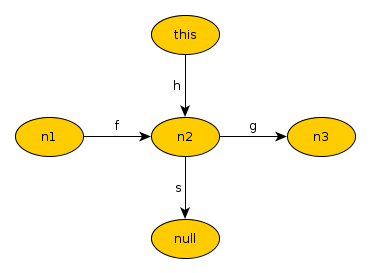
\includegraphics[scale=0.5]{ptg.png}
			\end{center}
			\caption{Points-to Graph de ejemplo}
			\end{figure}

			Si el Points-to Graph pertenece al método $m$, el único parámetro del mismo es $this$ y no devuelve nada, entonces:

			\begin{itemize}
				\item $escapes(m,\ n1)$ es falso porque no es alcanzable por $this$ ni por el scope global y no hay otros parámetros ni se devuelve nada.
				\item $escapes(m,\ n3)$ es verdadero porque $n3$ es alcanzable por $this$, que es un parámetro (implícito).
				\item $escapes\_through(m,\ n1,\ this.h)$ es falso.
				\item $escapes\_through(m,\ n3,\ this.h)$ es verdadero, porque $n3$ es alcanzable por $this.h.g$ y $this.h$ es subexpresión a izquierda de la misma.
				\item $escapes\_expr(m,\ this.h.s)$ es falso porque el nodo alcanzado por dicha expresión es nulo.
				\item $escapes\_expr(m,\ this.h.g)$ es verdadero.
				\item $escapes\_expr\_through\_expr(m,\ this.h,\ this.h.s)$ es falso porque ningún objeto escapa a través de $this.h.s$.
				\item $escapes\_expr\_through\_expr(m,\ this.h,\ this.h.g)$ es verdadero porque $this.h$ alcanza al nodo $n3$ que escapa por la expresión $this.h.g$.
			\end{itemize}

			En algunos casos el análisis de escape realiza sobre-aproximaciones y determina que ciertos nodos escapan del método cuando no lo hacen; para subsanar este incoveniente en la verificación, en todas las anotaciones de tiempo de vida, damos la posibilidad de omitir la verificación utilizando el parámetro \mono{trust}.

		\subsection{Verificación de \mono{DestTmp}}
			Para cada anotación \mono{Contract.Memory.DestTmp([bool trust])} en el método $m$ si \mono{trust} no es \mono{true}:

			Buscar el nodo $node$ correspondiente al próximo \textit{new} (es decir, el primer \textit{new} que ocurra después de la anotación) y verificar que $escapes(m,\ node)$ sea falso, es decir, que $node$ no escape de $m$. En caso de que escape generar una alerta que reporte que la anotación podría ser incorrecta.
		\subsection{Verificación de \mono{DestRsd}}
			Para cada anotación \mono{Contract.Memory.DestRsd(Contract.Memory.RsdType \\ rsd\_name [, bool trust])} en el método $m$ si \mono{trust} no es \mono{true}:

			Buscar el nodo $node$ correspondiente al próximo \textit{new} y verificar que $escapes(m,\ node)$ sea verdadero, es decir, que $node$ escape de $m$. En caso de que no escape generar una alerta que reporte que la anotación es incorrecta.

			Además en caso de que sí escape el nodo, tomar la expresión $expr$ asociada según el \mono{BindRsd} dado para el residual \mono{rsd\_name} y verificar que $escapes\_through(m,\ node,\ expr)$ sea verdadero, en caso de que no lo sea generar una alerta que reporte que la anotación es incorrecta.
		\subsection{Verificación de \mono{AddTmp}}
			Para cada anotación \mono{Contract.Memory.AddTmp(Contract.Memory.RsdType \\ rsd\_name\_call [, bool trust]);} en el método $m$ si \mono{trust} no es \mono{true}:

			Buscar según la expresión dada en \mono{BindRsd} del método llamado para el residual de nombre \mono{rsd\_name\_call} el objeto local al que escapa el residual del método llamado.

			Si la expresión es \mono{this} y la llamada es \mono{o.M()} entonces la expresión a evaluar es \mono{o}.

			Si la expresión es \mono{return} y la llamada es \mono{r = o.M()} entonces la expresión a evaluar es \mono{r}.

			Para el caso de los parámetros es necesario hacer un reemplazo del nombre utilizado en la expresión dada en \mono{BindRsd} por el nombre del objeto local pasado de parámetro. Por ejemplo, si la expresión es \mono{p.f} donde \mono{p} es el primer parámetro del método y la llamada es \mono{o.M(s)} entonces la expresión a evaluar es \mono{s.f}, porque el nombre de \mono{p} en el método llamador es \mono{s}. Esta misma lógica aplica si la expresión contiene a \mono{this}, pero el reemplazo a hacer en ese caso será de \mono{this} por el objeto sobre el que se invoca el método.

			Una vez obtenida esta expresión (llamémosla $expr$) verificar que $escapes\_expr(m,\ expr)$ sea falso, es decir, que el objeto correspondiente a $expr$ no escape del método. En caso de que no lo sea generar una alerta que reporte que la anotación podría ser incorrecta.

			\noindent Veamos un ejemplo:
			\vspace{5pt}
			\begin{footnotesize}
			\begin{lstlisting}[caption=Ejemplo de verificación de \mono{AddTmp}]
public void ProcesarLista(List<Nodo> lista, int tipo)
{
	Contract.Memory.Tmp<Nodo>(1);
	...
	Contract.Memory.AddTmp(Contract.Memory.Return);
	Nodo nodo = this.ProcesarNodo(nodo);
	...
}
			\end{lstlisting}
			\end{footnotesize}

			Para verificar la correctitud de la anotación de la línea 5 debemos buscar la expresión local asociada a la expresión \mono{return} del método \mono{ProcesarNodo} (el nombre de residual \mono{Contract.Memory.Return} se asocia siempre a la expresión \mono{return} que representa el objeto devuelto por el método). En este caso la expresión local es \mono{nodo}, entonces debemos verificar que $escapes\_expr(ProcesarLista,\ nodo)$ sea falso, es decir, que el objeto al que apunta \mono{nodo} no escape del método.

			Veamos otro ejemplo donde sea necesario hacer un reemplazo de nombres de acuerdo a la expresión dada en una anotación \mono{BindRsd}:

			\vspace{5pt}
			\begin{footnotesize}
			\begin{lstlisting}[caption=Ejemplo de verificación de \mono{AddTmp}]
Contract.Memory.RsdType rsd_ApilarElemento_pila;

public void ApilarElemento(Pila pila, int valor)
{
	Contract.Memory.BindRsd(rsd_ApilarElemento_pila, pila.Tope);
	Contract.Memory.Rsd<NodoPila>(rsd_ApilarElemento_pila, 1);
	...
	pila.Tope = new ElementoPila(valor);
	...
}

public void ProbarPila()
{
	Contract.Memory.Tmp<NodoPila>(1);
	...
	Pila pilaPrueba = new Pila();
	Contract.Memory.AddTmp(rsd_ApilarElemento_pila);
	this.ApilarElemento(pilaPrueba);
	...
}
			\end{lstlisting}
			\end{footnotesize}

		En el método \mono{ProbarPila} se indica que la memoria residual del método \mono{ApilarElemento} es transferida a la memoria temporal local, dicha memoria residual escapa del método \mono{ApilarElemento} a través de \mono{pila.Tope}, debemos reemplazar en esta expresión \mono{pila} por \mono{pilaPrueba} dado que ese es el parámetro pasado al método, entonces, para verificar la anotación \mono{AddTmp} del método \mono{ProbarPila} debemos verificar que $escapes\_expr(ProbarPila,\\ \ pilaPrueba.Tope)$ sea falso, es decir, que el objeto al que apunta \mono{pilaPrueba.Tope} no escape del método.

		\subsection{Verificación de \mono{AddRsd}}
			Para cada anotación \mono{Contract.Memory.AddRsd(Contract.Memory.RsdType \\ rsd\_name\_local, Contract.Memory.RsdType rsd\_name\_call [, bool trust]);} en el método $m$ si \mono{trust} no es \mono{true}:

			Buscar según la expresión dada en \mono{BindRsd} del método llamado para el residual de nombre \mono{rsd\_name\_call} el objeto local al que escapa el residual del método llamado usando la misma lógica descripta en la sección anterior.

			Una vez obtenida esta expresión (llamémosla $expr$) verificar que $escapes\_expr(m,\ expr)$ sea verdadero, es decir, que el objeto correspondiente a $expr$ escape del método. En caso de que no lo sea generar una alerta que reporte que la anotación es incorrecta.

			Además, en caso de que sí escape, tomar la expresión asociada según el \mono{BindRsd} dado para el residual \mono{rsd\_name\_local} en el método $m$ (llamémosla $expr\_local$) y verificar que $escapes\_expr\_through\_expr(m,\ expr,\ expr\_local)$ sea verdadero, en caso de que no lo sea generar una alerta que reporte que la anotación es incorrecta.

			\noindent Veamos un ejemplo:
			\vspace{5pt}
			\begin{footnotesize}
			\begin{lstlisting}[caption=Ejemplo de verificación de \mono{AddRsd}]
public void ProcesarLista(List<Nodo> lista, int tipo)
{
	Contract.Memory.Rsd<Nodo>(Contract.Memory.This, 1);
	...
	Contract.Memory.AddRsd(Contract.Memory.This, Contract.Memory.Return);
	this._head = this.ProcesarNodo(nodo);
	...
}
			\end{lstlisting}
			\end{footnotesize}

			En este caso, para verificar la correctitud de la anotación de la línea 5 debemos verificar dos cosas: primero, que el objeto transferido del método invocado (\mono{ProcesarNodo}) escape del método, y segundo, que si escapa, lo haga a través de la expresión asociada al residual local.

			Debemos buscar la expresión asociada al residual del método invocado, al igual que en el ejemplo anterior, el objeto escapa por \mono{return}, entonces la expresión asociada es \mono{this.\_head}.

			Primero verificamos que $escapes\_expr(ProcesarLista,\ this.\_head)$ sea verdadero, es decir, que el objeto al que apunta \mono{this.\_head} escape del método, en este caso lo será porque el nodo \mono{this} escapa por ser un parámetro. Luego debemos verificar que escape a través de la expresión asociada al residual \mono{Contract.Memory.This} que es \mono{this}, entonces verificamos que $escapes\_expr\_through\_expr(ProcesarLista,\ this.\_head,\ this)$ sea verdadero, que también lo será porque \mono{this.\_head} escapa a través de \mono{this}.

	\newpage
	\section{Incrementando las capacidades aritméticas de la verificación} \label{sec:mejbarv}
		Muchos verificadores estáticos (el de Code Contracts incluido) poseen un módulo aritmético con capacidades muy limitadas; la mayoría no son capaces de verificar la correctitud de relaciones entre expresiones donde aparecen multiplicaciones (por ejemplo, no son capaces de determinar la veracidad de $n^2 \geq n + 2\ \ \forall\ n \geq 2$). En general, sólo son capaces de verificar contratos con expresiones que tienen relaciones lineales.

		Como ya vimos en algunos ejemplos, es muy común que aparezcan multiplicaciones en los contratos de consumo de memoria, en el \autoref{ejrsdotros} la multiplicación surge de dos loops con el segundo dentro del primero, por lo tanto, para implementar una herramienta capaz de verificar todo tipo de contratos es necesario abordar esta problemática.

		En esta sección describimos un conjunto de instrumentaciones adicionales que apoyadas en el uso de alguna herramienta capaz de resolver operaciones aritméticas complejas permitirán incrementar las capacidades de verificación de la solución descripta hasta el momento para soportar contratos con expresiones no lineales.
		\subsection{Ejemplo motivacional}
			Comenzaremos mostrando un ejemplo para motivar la idea detrás de los algoritmos que describimos en las siguientes secciones.

			Dado el siguiente método:

			\vspace{15pt}
			\begin{footnotesize}
			\begin{lstlisting}[caption=Ejemplo motivacional para verificación de contratos con aritmética no lineal, label=ejverifbarv]
public void ConsumoCubicoCombinado(int n)
{
	Contract.Requires(n > 0);
	Contract.Memory.Tmp<C>(n * n * n);

	for (int i = 1; i <= n; i++)
	{
		for (int j = 1; j <= n; j++)
		{
			ConsumoCuadratico(i, j); // tiene un temporal de tipo C de i * j
		}
	}

	ConsumoCubico(n); // tiene un temporal de tipo C de n * n * n
}
			\end{lstlisting}
			\end{footnotesize}

			El contrato dado en el ejemplo es correcto, de la invocación de la línea 10 se debe obtener el máximo temporal en alguna de las invocaciones dentro de los dos loops, este máximo se da cuando \mono{i = n} y \mono{j = n}, dando así un temporal necesario de $n^2$, luego se debe calcular el máximo temporal entre $n^2$ y $n^3$ (producto de la invocación de la línea 14). Dicho máximo es $n^3$, por lo tanto el contrato es correcto. Sin embargo, el verificador de Code Contracts no es capaz de verificar la correctitud de este contrato\footnote{Esto sucede con la mayoría de los verificadores estáticos, dado que los mismos no están preparados para resolver aritmética si no para manejar aserciones lógicas.}.

			Supongamos que disponemos de un oráculo capaz de aseverar que ciertas relaciones son verdaderas (por ejemplo, que $max(n^2,\ n^3) = n^3$ es cierto $\forall\ n > 0$), y que esta información puede ser provista al verificador. La herramienta que utilizaremos para resolver las operaciones aritméticas complejas debe realizar el trabajo de este oráculo y la información que nos brinda la podemos inyectar en el código reemplazando algunas de las instrumentaciones descriptas en la Sección \hyperref[sec:verifcons]{\ref*{sec:verifcons} (Verificación de consumo mediante instrumentación)}, sumado a algunas asunciones que insertaremos, logrando así que el verificador utilizado verifique el contrato dado por el usuario.

			Las asunciones las insertaremos utilizando la anotación \mono{Contract.Assume} de Code Contracts (también disponible en otros lenguajes como JML y utilizada por otros verificadores), que recibe una expresión booleana que el verificador incorporará en su base de conocimiento durante la verificación asumiendo su correctitud, nos aseguraremos de proveer siempre expresiones correctas, en caso de no hacerlo podríamos generar una inconsistencia lógica.

			Notar que, como se desprenderá de los algoritmos presentados a continuación, es necesario que todos los loops sean anotados con el espacio de iteración utilizando la anotación \mono{Contract.Memory.IterationSpace}. En caso de no estar presente ésta en un loop, no se podrá hacer la verificación utilizando las técnicas que presentamos a continuación y se hará la instrumentación regular, descripta en secciones anteriores. En un futuro pensamos extraer el espacio de iteración calculado por el verificador (si es que lo calcula) para utilizarlo en estas técnicas de verificación.
		\subsection{Requisitos de la herramienta aritmética}
			La herramienta aritmética que utilicemos debe ser capaz de resolver las operaciones para polinomios con varias variables que definimos a continuación.

			$\mathbb{E}[\overline{P}]$ denota una expresión paramétrica entera en función de las variables del conjunto $\overline{P}$, por ejemplo:

				\begin{itemize}
					\item $\mathbb{E}[\overline{P}] = n^2 + m^2$ con $\overline{P} = \{n,\ m\}$.
					\item $\mathbb{E}[\overline{P}] = x + y$ con $\overline{P} = \{x\}$.
				\end{itemize}

			$\mathbb{E}_b[\overline{P}]$ denota una expresión paramétrica booleana en función de las variables del conjunto $\overline{P}$, por ejemplo:

				\begin{itemize}
					\item $\mathbb{E}_b[\overline{P}] = n^2 \geq 0$ con $\overline{P} = \{n\}$.
					\item $\mathbb{E}_b[\overline{P}] = 1 \leq x \leq y$ con $\overline{P} = \{x\}$.
				\end{itemize}

				\noindent Las operaciones que requerimos son:

				\begin{itemize}
					\item
						$count(inv,\ freeVars): \mathbb{E}_b[\overline{P}] \times \overline{P'} \mapsto \mathbb{E}[\overline{P'}]$ con $\overline{P'} \subseteq \overline{P}$

						\vspace{5pt}
						Cuenta la cantidad de puntos enteros restringidos a la expresión paramétrica $inv$ considerando a $\overline{P}$ como el conjunto variables libres en $inv$ (el resto de las variables son ligadas, para el uso que le daremos, por un ciclo), devolviendo una expresión paramétrica en función las variables libres.

						\vspace{5pt}
						\textbf{Ejemplo:} $count(1 \leq i \leq n\ \wedge\ 1 \leq j \leq m,\ \{n,\ m\}) = n * m$
					\item
						$maximize(e,\ inv,\ freeVars): \mathbb{E}[\overline{P}] \times \mathbb{E}_b[\overline{P}] \times \overline{P'} \mapsto \mathbb{E}[\overline{P'}]$ con $\overline{P'} \subseteq \overline{P}$
						
						\vspace{5pt}
						Determina el máximo valor entero que alcanza la expresión $e$ bajo las condiciones $inv$, considerando a $\overline{P}$ como el conjunto variables libres; devolviendo una expresión paramétrica que representa este valor máximo en función de las variables libres.

						\vspace{5pt}
						\textbf{Ejemplo:} $maximize(i * j,\ 1 \leq i \leq n\ \wedge\ 1 \leq j \leq m,\ \{n,\ m\}) = n * m$
					\item
						$summate(e,\ inv,\ freeVars): \mathbb{E}[\overline{P}] \times \mathbb{E}_b[\overline{P}] \times \overline{P'} \mapsto \mathbb{E}[\overline{P'}]$ con $\overline{P'} \subseteq \overline{P}$
						
						\vspace{5pt}
						Determina la suma de todos los puntos enteros de la expresión $e$ que cumplen las condiciones dadas por $inv$, considerando a $\overline{P}$ como el conjunto variables libres; devolviendo una expresión paramétrica que representa esta suma en función de las variables libres.

						\vspace{5pt}
						\textbf{Ejemplo:} $summate(i,\ 1 \leq i \leq n,\ \{n\}) = \frac{n * (n + 1)}{2}$
					\item
						$greater(e_1,\ \dots,\ e_n,\ inv): \mathbb{E}[\overline{P}] \times \dots \times \mathbb{E}[\overline{P}] \times \mathbb{E}_b[\overline{P}] \mapsto \mathbb{E}[\overline{P}] \times \mathbb{E}_b[\overline{P}]$
						
						\vspace{5pt}
						Determina cuál es la mayor expresión dentro de $e_1,\ \dots,\ e_n$ bajo las condiciones $inv$. Dado que esta expresión puede no ser única, el resultado podrá estar restringido a una condición que también es devuelta.

						\vspace{5pt}
						\textbf{Ejemplo 1:} $greater(n^2,\ n^3,\ n \geq 0) = (n^3,\ n \geq 0)$

						\vspace{5pt}
						\textbf{Ejemplo 2:} $greater(n^2,\ n + 2,\ n \geq 0) = (n^2,\ n \geq 2)$\footnote{Notar que en este caso existe más de un posible resultado, sin embargo, por el momento el prototipo desarrollado sólo es capaz de operar con uno solo.}
				\end{itemize}

		En nuestra implementación utilizaremos, para resolver las operaciones descriptas, la herramienta Barvinok \cite{barvinok}. Esta herramienta en particular soporta para las expresiones enteras sólo expresiones polinomiales (con varias variables) y para las expresiones booleanas sólo expresiones lineales (también con varias variables); sin embargo nada impide reemplazar esta herramienta en un futuro por otra con mayores capacidades.

		Definiremos una operación auxiliar para determinar las variables libres de un método. La operación $\mathit{FreeVars}(m)$ devuelve todas las subexpresiones a izquierda del cuerpo del método $m$ que comienzan con $this$ o con alguno de los parámetros del método y que no se modifican durante la ejecución del mismo. Por ejemplo, para el siguiente método:
		\vspace{5pt}
		\begin{lstlisting}[caption=Ejemplo de $\mathit{FreeVars}$]
public void BuscarElemento(List<Nodo> lista, Logger logger)
{
	logger.File.Open();
	logger.Log("Inicio");
	for (int i = 0; i < lista.Count; i++)
	{
		if (lista[i] == this.ElementoBuscado)
		{
			this.ElementoEncontrado = lista[i];
			logger.Log("Elemento encontrado");
			break;
		}
	}
	logger.File.Close();
}
		\end{lstlisting}

		En este caso $\mathit{FreeVars}(\mathit{BuscarElemento}) = \{this,\ lista,\ logger,\ logger.File,\\\ lista.Count,\ this.ElementoBuscado\}$

		En las siguientes secciones describimos la forma de utilizar las operaciones definidas para incrementar las capacidades de verificación de contratos con aritmética compleja para verificadores que no tienen estas capacidades.
		\subsection{Memoria temporal}
			Para un temporal de tipo \mono{T} en el método \mono{M} de la clase \mono{C} con los siguientes contratos:

			\mono{Contract.Memory.Tmp<T>(lim\_1, cond\_1);}

			\hspace{15pt}\vdots

			\mono{Contract.Memory.Tmp<T>(lim\_k, cond\_k);}

			\hspace{15pt}\vdots

			\mono{Contract.Memory.Tmp<T>(lim\_n, cond\_n);}

			Para este temporal anotado, en las siguientes subsecciones describimos cómo reemplazar, en caso de ser posible, la instrumentación descripta en la Sección \hyperref[sec:verifcons]{\ref*{sec:verifcons} (Verificación de consumo mediante instrumentación)} por una nueva instrumentación para tres casos: anotaciones adentro del cuerpo de loops, cálculo del máximo de memoria temporal de las invocaciones hechas y, finalmente, la verificación global (a nivel método) del contrato mismo.

			\subsubsection{Loops} \label{sec:loopsbarv}
				Para todos los loops anotados con \mono{IterationSpace}, consideremos a \mono{inv} como el espacio de iteración anotado en el loop; en caso de subloops, todos los subloops deben tener un espacio de iteración anotado y se debe considerar a \mono{inv} como todos ellos unidos por la operación lógica \textit{y}:
				\begin{itemize}
					\item
						Para cada \mono{DestTmp} donde el objeto creado en la línea siguiente es de tipo \mono{T}, en lugar de incrementar el contador correspondiente como se describió en los algoritmos de instrumentación, calcular:

						\begin{center}
						$cant\_directa\_loop\_i = count(inv,\ \mathit{FreeVars}(M))$
						\end{center}

						Es decir, la suma de la cantidad de veces que se hace un \textit{new} restringido al invariante. $i$ es el número de ocurrencia de este \mono{DestTmp} entre todos los loops.

						Luego, insertar después del loop más externo el statement:

						\begin{center}
						\mono{C\_M\_tmp\_T += cant\_directa\_loop\_i;}
						\end{center}
					\item
						Para cada invocación donde el método invocado tiene un contrato de memoria temporal de tipo \mono{T}, en lugar de hacer la instrumentación calcular:

						\begin{center}
						$max\_call\_loop\_i = maximize(tmp\_call,\ inv,\ \mathit{FreeVars}(M))$
						\end{center}

						Donde \textit{i} es el número de invocación entre todos los loops y $tmp\_call$ es la expresión del temporal de tipo \mono{T} del método llamado (asumimos que es único, no se soportan en este caso contratos de memoria temporal con condiciones dado que implica una explosión exponencial en la instrumentación\footnote{Una alternativa es tomar el máximo entre todos los contratos, sin embargo esto no siempre es posible y puede generar una pérdida de precisión importante; por esta razón en estos casos se realiza la instrumentación regular que en algunos casos es verificable.}).

						Esta expresión calcula el máximo valor que puede alcanzar la memoria temporal dentro del loop, reemplazando el máximo calculado en la instrumentación regular con \mono{Math.Max}.

						Luego, insertar afuera del loop más externo:

						\begin{center}
						\mono{max\_i\_T = max\_call\_loop\_i;}
						\end{center}

						Donde \mono{max\_i\_T} es la variable insertada antes del loop por la instrumentación explicada anteriormente en la Sección \hyperref[sec:callsloops]{\ref*{sec:callsloops} (Invocaciones dentro de loops)} utilizada para calcular el máximo de todas las invocaciones dentro de loops.
					\item
						Para cada \mono{AddTmp(rsd)} donde existe un residual de nombre \mono{rsd} y tipo \mono{T} en el siguiente método invocado, en lugar de insertar la suma correspondiente calcular:

						\begin{center}
						$cant\_transf\_loop\_i = summate(rsd\_call,\ inv,\ \mathit{FreeVars}(M))$
						\end{center}

						Donde \textit{i} es el número de \mono{AddTmp} entre todos los loops y \textit{rsd\_call} es la expresión del residual con nombre \mono{rsd} y tipo \mono{T} del método llamado (al igual que con los temporales, no se soportan residuales con condiciones).

						Esta expresión calcula la suma de memoria residual transferida del método llamado al temporal local.

						Luego, insertar afuera del loop más externo:

						\begin{center}
						\mono{C\_M\_tmp\_T += cant\_transf\_loop\_i;}
						\end{center}
				\end{itemize}
			\subsubsection{Máximo de memoria temporal de invocaciones}
				En la Sección \hyperref[sec:callsfueraloops]{\ref*{sec:callsfueraloops} (Invocaciones fuera de loops)} describimos en la ecuación $(1)$ el incremento del contador correspondiente al temporal de tipo \mono{T} con el máximo de los temporales de todas las invocaciones hechas (recordar que a este máximo luego se incorporan los máximos calculados dentro de loops).

				El verificador de Code Contracts no es capaz de resolver esta maximización para casos no lineales o con más de una variable involucrada, pero utilizando las operaciones definidas podremos resolverla correctamente.

				Si para todas las invocaciones hechas dentro de loops se pudo calcular un polinomio que represente el consumo de memoria temporal dentro de ese loop, entonces se tendrán una serie de expresiones $tmp_1,\ \dots\ ,\ tmp_n$ que representan el requerimiento de memoria temporal de todos los métodos invocados; en ese caso, podemos calcular:

					\begin{center}
					$max\_calls = greater(tmp_1,\ \dots\ ,\ tmp_n,\ inv)$
					\end{center}

				Donde $inv$ son todas las precondiciones en los contratos del método (condiciones dadas con \mono{Contract.Requires}).

				Y luego reemplazar la instrumentación hecha en $(1)$ por:

					\begin{center}
					\mono{C\_M\_tmp\_T += max\_calls;}
					\end{center}

				Este incremento puede estar restringido a una condición, en cuyo caso lo hacemos bajo un \mono{if} y si no se cumple la condición hacemos que falle la verificación insertando una anotación \mono{Contract.Assert(false);}.

				En el \autoref{ejverifbarv} presentado al comienzo de la sección se debería calcular el máximo de $n^2$, calculado usando el segundo algoritmo de la Sección \hyperref[sec:loopsbarv]{\ref*{sec:loopsbarv} (Loops)} y $n^3$, resultado de la llamada a \mono{ConsumoCubico}. Usando $greater$ obtenemos que este máximo es $n^3$ siempre que \mono{n >= 0} por lo que insertamos el siguiente código en lugar de la instrumentación:

				\vspace{15pt}
				\begin{lstlisting}[caption=Ejemplo de código insertado de máximo calculado con $greater$]
if (n >= 0)
{
	C_M_tmp_T += n * n * n;
}
else
{
	Contract.Assert(false);
}
				\end{lstlisting}

				En caso de que no se cumpla la condición hacemos que falle la verificación usando \mono{Contract.Assert(false)} porque no sabemos qué sucede con el contador dado que la herramienta aritmética no fue capaz de calcularlo.

				Notar que esta instrumentación pierda la sensibilidad a flujo para el análisis y genera una sobre-aproximación, en futuras versiones pensamos solucionar este problema.

			\subsubsection{Verificación global}
				Con las instrumentaciones descriptas hasta el momento, se insertan en el código varios resultados pre-calculados que muchos verificadores no son capaces de calcular; sin embargo, aún existirán contratos que no serán capaces de ser verificados. Supongamos el siguiente método:

				\vspace{15pt}
				\begin{small}
				\begin{lstlisting}[caption=Ejemplo de contrato no verificable por Code Contracts]
public void ConsumoCubico(int n)
{
	Contract.Requires(n >= 2);
	Contract.Memory.Tmp<C>(n * n * n);

	for (int i = 1; i <= n; i++)
	{
		Contract.Memory.DestTmp();
		C c = new C();
	}

	ConsumoCuadratico(n); // tiene un temporal de tipo C de n * n
}
				\end{lstlisting}
				\end{small}

				El consumo exacto de este método es $n + n^2$ ($n$ en el loop y $n^2$ en la invocación de la línea 12), dado que $n^3 \geq n^2 + n\ \ \forall\ n \geq 2$ el contrato dado en el método es correcto; sin embargo contiene una relación no lineal.

				Utilizaremos las funciones definidas para intentar verificar la correctitud del contrato con el oráculo, y en caso de ser cierto insertaremos un \mono{Contract.Assume} que perimitará al verificador verificar el contrato. Lo que hacemos en este caso es adelantar la verificación, y en caso de poder hacerla le informamos al verificador mediante el \mono{Contract.Assume} que el contrato es correcto.

				En rasgos generales, generaremos una expresión resultado de la suma de todas las expresiones en que se incrementa el contador \mono{C\_M\_tmp\_T} para luego verificar con la herramienta aritmética si dicha expresión es menor o igual que la expresión dada en el contrato, teniendo en cuenta las posibles condiciones dadas para cada contrato. A continuación describimos en detalle la forma en que esto se debe implementar.

				Sean las siguientes expresiones:
				\begin{itemize}
					\item
						$cant\_directa\_loop\_i$: definido anteriormente, es la cantidad de \mono{DestTmp} hechas adentro de loops.

						$i$ va desde 1 hasta $num\_DestTmp$, el número total de \mono{DestTmp} anotados en el método.
					\item
						$max\_call\_loop\_i$: definido anteriormente, es el máximo de cada invocación adentro de loops.

						$i$ va desde 1 hasta $num\_CallsLoops$, el número total de invocación hechas dentro de loops.
					\item
							$cant\_transf\_loop\_i$: definido anteriormente, es la cantidad de temporal transferida desde residuales al temporal local adentro de loops.

							$i$ va desde 1 hasta $num\_AddTmpLoops$, el número total de \mono{AddTmp} anotados en el método dentro de loops.
					\item
						$cant\_directa$: cantidad de news de tipo \mono{T} hechos fuera de loops anotados con \mono{DestTmp}.
					\item
						$tmp\_call\_i$: es la cantidad de memoria temporal de tipo \mono{T} de las invocaciones fuera de loops (\mono{i} es el número de invocación fuera de loops).

						$i$ va desde 1 hasta $num\_Calls$, el número total de invocaciones hechas fuera de loops.
					\item
						$cant\_transf\_i$: es la cantidad de temporal transferida desde residuales al temporal local fuera de loops (\mono{i} es el número de invocación fuera de loops).

						$i$ va desde 1 hasta $num\_AddTmp$, el número total de \mono{AddTmp} anotados en el método fuera de loops.
				\end{itemize}

				Sea la expresión:

					$$cand\_tmp = \sum_{i=1}^{num\_DestTmp}{cant\_directa\_loop\_i}\ +\ cant\_directa\ +\ $$

					$$\sum_{i=1}^{num\_AddTmpLoops}{cant\_transf\_loop\_i}\ +\ \sum_{i=1}^{num\_AddTmp}{cant\_transf\_i}\ +\ $$

					$$greater(max\_call\_loop\_1,\ \dots,\ max\_call\_loop\_num\_CallsLoops,\ $$

					$$tmp\_call\_1,\ \dots,\ tmp\_call\_num\_Calls,\ preconditions)$$

				Donde $preconditions$ son las precondiciones del método \mono{M}.

				$cand\_tmp$ es la suma de la memoria consumida directamente por \textit{news} (dentro y fuera de loops), más la memoria transferida de residuales de invocaciones al temporal local (dentro y fuera de loops) más el máximo de memoria temporal de todas las invocaciones hechas (dentro y fuera de loops).

				Calcular para cada $1 \leq k \leq n$:

				\begin{center}
				$max = greater(cand\_tmp,\ lim\_k,\ cond\_k)$
				\end{center}

				En caso de no haber una condición, utilizar $true$ como invariante.

				Si se determina que $max = lim\_k$, es decir, se cumple que $cand\_tmp \leq lim\_k$ bajo $cond\_k$, insertar el statement:

				\vspace{5pt}
				\begin{lstlisting}[numbers=none]
Contract.Assume(C_M_tmp_T <= lim_k);
				\end{lstlisting}

				Si se determina que $max = lim\_k$ bajo ciertas condiciones \mono{conds}, insertar el statement:

				\vspace{5pt}
				\begin{lstlisting}[numbers=none]
if (conds)
{
	Contract.Assume(C_M_tmp_T <= lim_k);
}
else
{
	Contract.Assert(false);
}
				\end{lstlisting}

				De esta forma, el verificador podrá utilizar estos assumes para determinar la correctitud de los contratos dados por el usuario, siempre y cuando se cumplan las condiciones, caso contrario fallará la verificación.
		\subsection{Memoria residual}
			Las instrumentaciones y verificaciones hechas para la memoria residual son muy similares a las presentadas para la memoria temporal, pero sin tener el cuenta el cálculo del máximo de la memoria requerida por los métodos invocados.

			Para un residual de tipo \mono{T} y nombre \mono{rsd\_local} en el método \mono{M} de la clase \mono{C} con los siguientes contratos:

			\mono{Contract.Memory.Rsd<T>(rsd\_local, lim\_1, cond\_1);}

			\hspace{15pt}\vdots

			\mono{Contract.Memory.Rsd<T>(rsd\_local, lim\_k, cond\_k);}

			\hspace{15pt}\vdots

			\mono{Contract.Memory.Rsd<T>(rsd\_local, lim\_n, cond\_n);}

			Para este residual anotado, en las siguientes subsecciones describimos cómo reemplazar, en caso de ser posible, la instrumentación descripta en la Sección \hyperref[sec:verifcons]{\ref*{sec:verifcons} (Verificación de consumo mediante instrumentación)} por una nueva instrumentación para dos casos: anotaciones adentro del cuerpo de loops y la verificación global (a nivel método) del contrato mismo.

			\subsubsection{Loops}
				Para todos los loops anotados con \mono{IterationSpace}, consideremos a \mono{inv} como el espacio de iteración anotado en el loop; en caso de subloops, todos los subloops deben tener un espacio de iteración anotado y se debe considerar a \mono{inv} como todos ellos unidos por la operación lógica \textit{y}:
				\begin{itemize}
					\item
						Para cada \mono{DestRsd(rsd\_local)} donde el objeto creado en la línea siguiente es de tipo \mono{T}, en lugar de incrementar el contador correspondiente como se describió en los algoritmos de instrumentación, calcular:

						\begin{center}
						$cant\_directa\_loop\_i = count(inv,\ \mathit{FreeVars}(M))$
						\end{center}

						Es decir, la suma de la cantidad de veces que se hace un \textit{new} restringido al invariante. $i$ es el número de ocurrencia de este \mono{DestRsd(rsd\_local)} entre todos los loops.

						Luego, insertar después del loop más externo el statement:

						\begin{center}
						\mono{C\_M\_rsd\_local\_T += cant\_directa\_loop\_i;}
						\end{center}
					\item
						Para cada \mono{AddRsd(rsd\_local, rsd\_method)} donde existe un residual de nombre \mono{rsd\_method} y tipo \mono{T} en el siguiente método invocado, en lugar de insertar la suma correspondiente calcular:

						\begin{center}
						$cant\_transf\_loop\_i = summate(rsd\_call,\ inv,\ \mathit{FreeVars}(M))$
						\end{center}

						Donde \textit{i} es el número de \mono{AddRsd(rsd\_local)} entre todos los loops y \textit{rsd\_call} es la expresión del residual con nombre \mono{rsd} y tipo \mono{T} del método llamado (al igual que con los temporales, no se soportan residuales con condiciones).

						Esta expresión calcula la suma de memoria residual transferida del método llamado al residual local.

						Luego, insertar afuera del loop más externo:

						\begin{center}
						\mono{C\_M\_rsd\_local\_T += cant\_transf\_loop\_i;}
						\end{center}
				\end{itemize}
			\subsubsection{Verificación global}
				De la misma forma que con la memoria temporal, hacemos una verificación de los contratos e insertamos los \mono{Contract.Assume} correspondientes en caso de poder hacerlo.

				En rasgos generales, generaremos una expresión resultado de la suma de todas las expresiones en que se incrementa el contador \mono{C\_M\_rsd\_local\_T} para luego verificar con la herramienta aritmética si dicha expresión es menor o igual que la expresión dada en el contrato, teniendo en cuenta las posibles condiciones dadas para cada contrato. A continuación describimos en detalle la forma en que esto se debe implementar.

				Sean las siguientes expresiones:
				\begin{itemize}
					\item
						$cant\_directa\_loop\_i$: definido anteriormente, es la cantidad de \\ \mono{DestRsd(rsd\_local)} hechas adentro de loops.

						$i$ va desde 1 hasta $num\_DestRsd$, el número total de \mono{DestRsd} anotados en el método.
					\item
						$cant\_transf\_loop\_i$: definido anteriormente, es la cantidad de residual transferida desde residuales al residual local adentro de loops.

						$i$ va desde 1 hasta $num\_AddRsdLoops$, el número total de \mono{AddRsd} anotados en el método dentro de loops.
					\item
						$cant\_directa$: cantidad de news de tipo \mono{T} hechos fuera de loops anotados con \mono{DestRsd(rsd\_local)}.
					\item
						$cant\_transf\_i$: es la cantidad de residual transferida desde residuales al residual local fuera de loops (\mono{i} es el número de invocación fuera de loops).

						$i$ va desde 1 hasta $num\_AddRsd$, el número total de \mono{AddRsd} anotados en el método fuera de loops.
				\end{itemize}
				
				Sea la expresión:

					$$cand\_rsd = \sum_{i=1}^{num\_DestRsd}{cant\_directa\_loop\_i}\ +\ cant\_directa\ +\ $$

					$$\sum_{i=1}^{num\_AddRsdLoops}{cant\_transf\_loop\_i}\ +\ \sum_{i=1}^{num\_AddRsd}{cant\_transf\_i}$$

				$cand\_rsd$ es la suma de la memoria consumida directamente por \textit{news} (dentro y fuera de loops) más la memoria transferida de residuales de invocaciones al residual local (dentro y fuera de loops).

				Calcular para cada $1 \leq k \leq n$:

				\begin{center}
				$max = greater(cand\_rsd,\ lim\_k,\ cond\_k)$
				\end{center}

				En caso de no haber una condición, utilizar $true$ como invariante.

				Si se determina que $max = lim\_k$, es decir, se cumple que $cand\_rsd \leq lim\_k$ bajo $cond\_k$, insertar el statement:

				\vspace{5pt}
				\begin{lstlisting}[numbers=none]
Contract.Assume(C_M_rsd_local_T <= lim_k);
				\end{lstlisting}

				Si se determina que $max = lim\_k$ bajo ciertas condiciones \mono{conds}, insertar el statement:

				\vspace{5pt}
				\begin{lstlisting}[numbers=none]
if (conds)
{
	Contract.Assume(C_M_rsd_local_T <= lim_k);
}
else
{
	Contract.Assert(false);
}
				\end{lstlisting}

				De esta forma, el verificador podrá utilizar estos assumes para determinar la correctitud de los contratos dados por el usuario, siempre y cuando se cumplan las condiciones, caso contrario fallará la verificación.

	\newpage
	\section{Overview de la implementación} \label{sec:overimpl}
		\subsection{Arquitectura genérica}
			Comenzaremos primero describiendo la arquitectura de la solución genéricamente sin tener en cuenta la implementación particular hecha, describiendo los requerimientos de cada componente. Luego, en las siguientes secciones detallamos la arquitectura de la herramienta desarrollada.

			\begin{figure}[htb]
			\begin{center}
			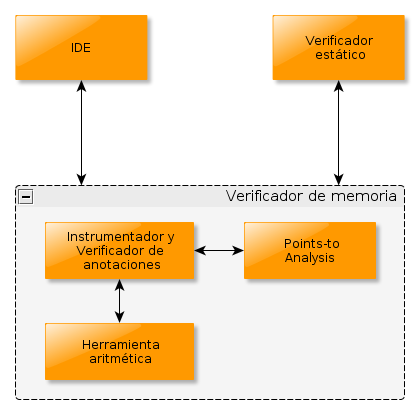
\includegraphics[scale=0.5]{arqgeneral.png}
			\end{center}
			\caption{Arquitectura genérica}
			\label{arqgen}
			\end{figure}

			En la Figura \ref{arqgen} vemos la arquitectura genérica de la solución propuesta a lo largo del trabajo.

			En la Figura \ref{seqarq} vemos un diagrama de secuencia que describe el flujo del control durante la verificación. La IDE es la encargada de iniciar la verificación luego de la compilación del código. Según la plataforma, la IDE enviará al verificador de memoria el código compilado o el código fuente, luego el verificador de memoria hará la verificación y devolverá a la IDE el resultado de la verificación para que sea mostrada al usuario.

			El verificador de memoria realiza la instrumentación del código y la verificación de anotaciones como se describió en las secciones anteriores, utilizando el análisis de points-to y escape para obtener información del tiempo de vida de los objetos y la herramienta aritmética para enriquecer el código instrumentado con información que ayude a la verificación.

			El código instrumentado es enviado al verificador estático, el cual verifica la correctitud de los nuevos contratos insertados y devuelve los resultados al verificador de memoria, éste deberá agregar a estos resultados los de la verificación de anotaciones hecha para devolverlos a la IDE.

			\begin{figure}[htb]
			\begin{center}
			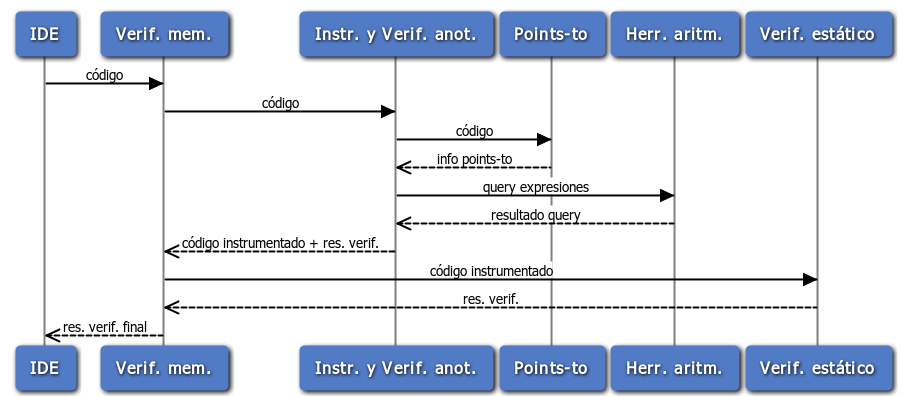
\includegraphics[scale=0.5]{seqdiag_arq.png}
			\end{center}
			\caption{Diagrama de secuencia mostrando el flujo del control durante la verificación}
			\label{seqarq}
			\end{figure}

			A partir de ahora nos concentraremos en explicar la forma en que esta arquitectura se utilizó en la implementación de prueba de concepto hecha para este trabajo, utilizando Microsoft Visual Studio como IDE, el verificador de Code Contracts como verificador estático y como verificador de memoria una implementación de los algoritmos descriptos junto a la herramienta aritmética Barvinok y el análisis de points-to y escape de \cite{BFGL07}.
		\subsection{Plataforma y herramientas utilizadas}
			Como ya mencionamos, hicimos una implementación de la solución propuesta para la plataforma .NET usando el analizador estático de la herramienta Code Contracts (Clousot, \cite{Ff10}). Elegimos esta plataforma y herramienta dado que son activamente desarrolladas y mantenidas en la actualidad, además tienen una sintaxis para escribir anotaciones muy intuitiva e integrada con la IDE (Microsoft Visual Studio) que fácilmente podemos extender para soportar nuestras nuevas anotaciones.

			El verificador estático de Code Contracts (Clousot) utiliza técnicas de interpretación abstracta para intentar demostrar la correctitud de los contratos, a diferencia de los verificadores estáticos más comunes que se basan en calcular y demostrar la precondición más débil. El uso de interpretación abstracta permite al verificador inferir automáticamente los invariantes de ciclo e integrar en la verificación diferentes heurísticas para ajustar el tradeoff entre el costo de la verificación y su precisión.

			Dado que en Code Contracts los contratos son código embebido, pudimos extender estos contratos permitiendo al usuario escribir los nuevos contratos de consumo de memoria de la misma forma que lo harían con contratos de Code Contracts, aprovechando las ventajas que la IDE brinda, tales como documentación inline mientras se escriben las anotaciones y chequeo de tipos y sintaxis de las mismas.

			Una ventaja importante es que la plataforma .NET cuenta con un framework para análisis estático e instrumentación de código llamada \mono{CCI} (Common Compiler Infraestructure: \cite{CCImeta}, \cite{CCIast}) que es de código abierto, tiene buena documentación de uso y soporte nativo para inyectar contratos de Code Contracts.

			Otra característica interesante de Code Contracts es que todos los contratos escritos por el usuario quedarán embebidos en el código compilado, por lo que al distribuirlo se estarán proveyendo contratos de consumo de memoria en caso de que el código estuviese anotado; también es posible distribuir los contratos y el código en archivos separados.
		\subsection{Arquitectura de la solución implementada}
			Para comprender la arquitectura de la herramienta desarrollada y el flujo de los elementos entre sus diferentes partes, es primero conveniente conocer la forma en que funciona la verificación estática hecha por Code Contracts, dado que nuestra solución es una extensión de la misma.

			\begin{figure}[htb]
			\begin{center}
			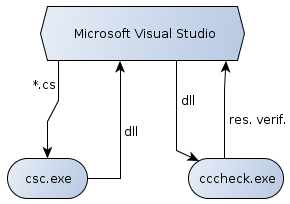
\includegraphics[scale=0.5]{arq_cc.png}
			\end{center}
			\caption{Arquitectura de la verificación estática de Code Contracts}
			\label{arqcc}
			\end{figure}

			 La verificación comienza cuando el usuario compila el código en la IDE (Ver Figura \ref{arqcc}). Todos los archivos con extensión \mono{cs} (asumiendo código C\#) de un mismo proyecto son enviados al compilador \mono{csc.exe} que devuelve una \mono{dll} con el código compilado, luego, en caso de tener activada la verificación estática, esta \mono{dll} es enviada al verificador estático de Code Contracts llamado \mono{cccheck.exe} el cual analiza los contratos, intenta verificarlos y devuelve el resultado a la IDE (este resultado es un texto con un formato acordado) la cual muestra los resultados al usuario en una forma amigable. Vale aclarar que este proceso se realiza por separado para cada proyecto compilado (un proyecto equivale a una \mono{dll} o assembly en .NET).

			La extensión que hacemos del verificador nativo, en rasgos generales, intercepta la \mono{dll} antes de que sea enviada a \mono{cccheck.exe}, la analiza y modifica y luego la envía a \mono{cccheck.exe}, tomando su salida para devolvérsela a la IDE agregándole resultados de ciertas verificaciones hechas. En la Figura \ref{arqccmem} se puede ver la arquitectura, ahora explicaremos en detalle el flujo de la información en esta arquitectura y la responsabilidad de cada componente. Los números entre paréntesis indican el orden dentro del flujo del control durante la ejecución.

			\begin{figure}[htb]
			\begin{center}
			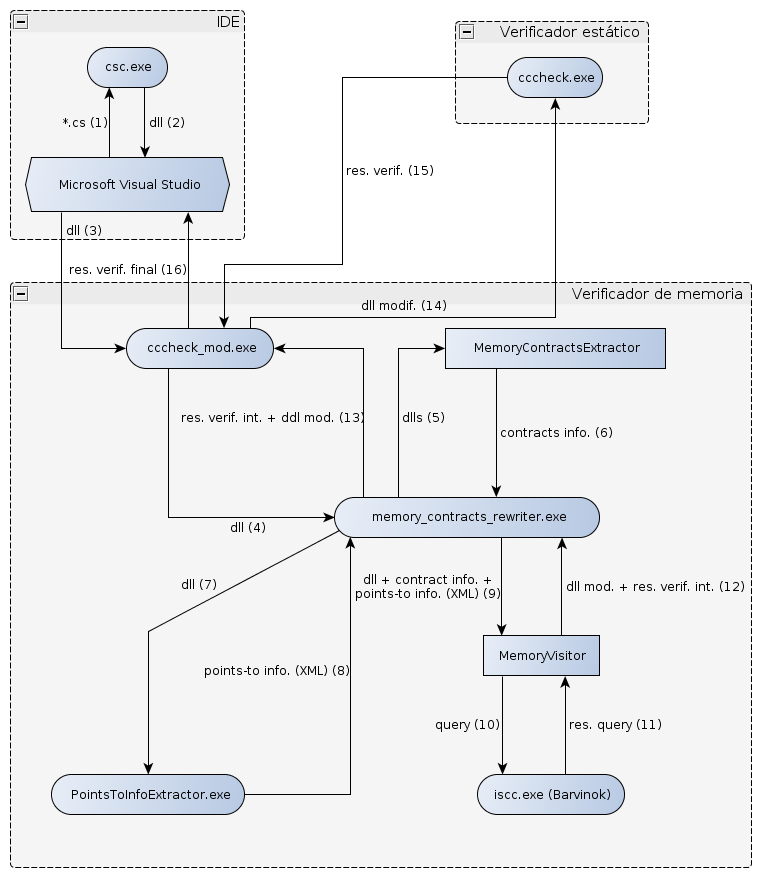
\includegraphics[scale=0.5]{arq_cc_mem.png}
			\end{center}
			\caption{Arquitectura de la verificación estática de Code Contracts con memoria}
			\label{arqccmem}
			\end{figure}

			Al igual que en el caso anterior, la verificación comienza cuando el usuario compila el código en la IDE, luego de enviarse al compilador (1) y obtener la \mono{dll} (2) ésta es enviada a verificar. Modificando la configuración de Code Contracts es posible hacer que la IDE envíe la \mono{dll} a verificar a nuestro componente, llamado \mono{cccheck\_mod.exe} en lugar de al componente de Code Contracts (3). Dado que este componente respeta la misma interfaz que \mono{cccheck.exe} (recibe una \mono{dll} y devuelve en la salida estándar un texto con el resultado de la verificación), el cambio es transparente para la IDE.

			Lo siguiente que hace \mono{cccheck\_mod.exe} es enviar la \mono{dll} al componente llamado \mono{memory\_contracts\_rewriter.exe} (4), éste es el componente central de nuestra herramienta, encargado de coordinar la instrumentación del código y verificación de las anotaciones. El mismo se encarga de parte de la verificación pero no toda, dado que la correctitud de ciertas anotaciones es verificada por este componente (por ejemplo de \mono{DestTmp} y \mono{DestRsd}) mientras que otras (como los contratos) son transformadas en contratos nativos de Code Contracts que luego \mono{cccheck.exe} verificará gracias a la instrumentación de código hecha.

			\mono{memory\_contracts\_rewriter.exe} primero extrae de la \mono{dll}, utilizando otras componentes, un conjunto de información necesaria para la siguiente tarea. Utilizando la clase \mono{MemoryContractsExtractor} (5 y 6), implementada con \mono{CCI}, extrae los contratos de memoria de la \mono{dll} y de todas las \mono{dlls} a las que ésta referencia (notar que si en un futuro los contratos se distribuyen separados de las \mono{dlls} compiladas, se debería modificar sólo esta clase). Además, utilizando el componente \mono{PointsToInfoExtractor.exe} obtiene un Points-to Graph junto con información de escape (en formato XML) de todos los métodos de la \mono{dll} (7 y 8). Este componente está basado en un análisis disponible en \mono{CCI} hecho por Diego Garbervetsky para Spec\#, implementado según \cite{BFGL07}.

			Luego, una vez recolectada esta información, la misma junto a la \mono{dll} original se envía a la clase \mono{MemoryVisitor} (9), esta clase está implementada con \mono{CCI} y se encarga de analizar cada método de cada clase contenida en la \mono{dll}, este análisis realiza tres tareas principales:
				\begin{itemize}
					\item Hace la instrumentación de código necesaria e inserción de contratos de Code Contracts (generados a partir de contratos de memoria), para la posterior verificación. Para esto se utilizan los algoritmos descriptos en la Sección \hyperref[sec:verifcons]{\ref*{sec:verifcons} (Verificación de consumo mediante instrumentación)}.
					\item Verifica la correctitud de otras anotaciones que no pueden ser verificadas por \mono{cccheck.exe}. Estas verificaciones se realizan utilizando las técnicas descriptas en la Sección \hyperref[sec:verifcorr]{\ref*{sec:verifcorr} (Verificación de correctitud de las anotaciones de tiempo de vida)}.
					\item Haciendo uso de \mono{iscc.exe} (la calculadora de la herramienta \mono{Barvinok}) se intenta obtener aserciones sobre el consumo de memoria que son inyectadas en el código junto a los contratos (10 y 11), ayudando así a la posterior verificación; se utilizan para estos los algoritmos descriptos la Sección \hyperref[sec:mejbarv]{\ref*{sec:mejbarv} (Incrementando las capacidades aritméticas de la verificación)}.
				\end{itemize}
			Para todos los ítems se utiliza la información de contratos extraida anteriormente y para el segundo se utiliza la información de points-to y escape. Como resultado de todo el proceso se obtiene una nueva \mono{dll} con código instrumentado y nuevos contratos insertados, y un conjunto de aserciones resultado de las verificaciones hechas en el segundo punto.

			Esta \mono{dll} modificada y las aserciones son devueltas a \mono{memory\_contracts\_rewriter.exe} (12) el cual a su vez las devuelve a \mono{cccheck\_mod.exe} (13), éste envía la \mono{dll} modificada a \mono{cccheck.exe} (14) el cual hace la verificación de los nuevos contratos generados y devuelve el resultado (15), este resultado es unido al resultado de la verificación hecha en \mono{MemoryVisitor} (llamado \mono{res. verif. int.} en el diagrama) y finalmente devuelto a la IDE (16) que muestra los resultados de la verificación hecha por \mono{cccheck.exe} del código instrumentado junto a las verificaciones hechas por \mono{MemoryVisitor} directamente.

	\newpage
	\section{Evaluación} \label{sec:exp}
		En esta sección mostramos una serie de experimentos hechos utilizando la herramienta desarrollada para evaluar sus capacidades. A lo largo de los mismos veremos la forma en que se realiza la instrumentación y verificación para cada uno de ellos y observaremos algunas limitaciones de la herramienta.

		Todos los experimentos consisten en una o más clases con sus métodos anotados con contratos de consumo de memoria y otras anotaciones necesarias para la verificación. Veremos en algunos casos el código instrumentado y en otros analizaremos la forma en la que la misma es resuelta por el verificador.
		\subsection{Verificación en el ejemplo dado en el Anexo}
			Veremos la forma en que se realiza la instrumentación para algunos métodos de las clases presentadas en la Sección \hyperref[sec:ejcompanot]{\ref*{sec:ejcompanot} (Ejemplo completo anotado)} del Anexo.

			El ejemplo dado en el Anexo consiste de cuatro clases (\mono{Address}, \mono{AddressValidator}, \mono{Person} y \mono{PeopleManager}). Todos los contratos del mismo son verificables por la herramienta desarrollada y cubre todos los tipos de anotaciones disponibles. Veremos la instrumentación de un método utilizando las técnicas de la Sección \hyperref[sec:verifcons]{\ref*{sec:verifcons} (Verificación de consumo mediante instrumentación)} y la de otro usando las técnicas de la Sección \hyperref[sec:mejbarv]{\ref*{sec:mejbarv} (Incrementando las capacidades aritméticas de la verificación)}.

			El método \mono{CreateFamily} de la clase \mono{PeopleManager} no puede ser instrumentado utilizando las técnicas de la Sección \hyperref[sec:mejbarv]{\ref*{sec:mejbarv} (Incrementando las capacidades aritméticas de la verificación)} dado que tiene un ciclo que no está anotado con el espacio de iteración, sin embargo puede ser verificado con la instrumentación regular porque sus contratos sólo tienen expresiones lineales. El siguiente es el código de dicho método instrumentado (los nombres de los campos para contadores se renombraron por cuestiones de espacio):

			\vspace{15pt}
			\begin{scriptsize}
			\begin{lstlisting}[caption=Método \mono{CreateFamily} instrumentado]
public static Person[] CreateFamily(List<string> firstNames, string lastName, string street, string city, string state)
{
    Contract.Requires(firstNames.Count > 0);
    Contract.Ensures(tmp_AddressValidator <= 1);
    Contract.Ensures(rsd_Return_Address <= firstNames.Count);
    Contract.Ensures(rsd_Return_Person <= firstNames.Count);
    Contract.Ensures(rsd_Return_Person_arr <= 1);
    rsd_Return_Address = 0;
    rsd_Return_Person = 0;
    rsd_Return_Person_arr = 0;
    int tmp_call_1 = 0;
    tmp_AddressValidator = 0;
    Contract.Memory.Rsd<Person>(Contract.Memory.Return, firstNames.Count);
    Contract.Memory.Rsd<Person[]>(Contract.Memory.Return, 1);
    Contract.Memory.Rsd<Address>(Contract.Memory.Return, firstNames.Count);
    Contract.Memory.Tmp<AddressValidator>(1);
    
    Contract.Memory.DestRsd(Contract.Memory.Return);
    rsd_Return_Person_arr++;
    Person[] family = new Person[firstNames.Count];
    
    for (int i = 0; i < firstNames.Count; i++)
    {
        Contract.Memory.AddRsd(Contract.Memory.Return, Contract.Memory.This);
        Contract.Memory.DestRsd(Contract.Memory.Return);
        rsd_Return_Person++;
        Person person = new Person(firstNames[i], lastName, street, city, state);
        rsd_Return_Address += Person.rsd_This_Address;
        tmp_call_1 = Math.Max(tmp_call_1, Person.tmp_AddressValidator);
        family[i] = person;
    }
    tmp_AddressValidator += tmp_call_1;
    return family;
}
			\end{lstlisting}
			\end{scriptsize}

			En las líneas 4 a 7 se ven los contratos insertados por la herramienta, luego en las líneas 8 a 12 se ve la inicialización de los contadores en 0 y la declaración de la variable local \mono{tmp\_call\_1} que será utilizada para calcular el máximo del temporal de la invocación de la línea 27 (el \textit{new}).

			Adentro del loop, se incrementan los contadores correspondientes a la creación del objeto \mono{Person} en la línea 24 y de la transferencia del residual del método llamado al residual local. En la línea 29 se encuentra la instrumentación hecha con \mono{Math.Max} para calcular el máximo temporal consumido por la invocación dentro del loop. Este máximo queda al final del loop en la variable \mono{tmp\_call\_1} que es sumada el contador correspondiente luego del loop.

			Hemos comprobado que este tipo de instrumentación utilizando \mono{Math.Max} no funciona para loops anidados o con un espacio de iteración complejo cuando la verificación se hace con el verificador de Code Contracts, para poder verificar contratos bajo esas condiciones es necesario anotar los espacios de iteración, como veremos en el siguiente ejemplo.

			Uno de los métodos más complejos en este conjunto de clases es el método\\ \mono{CreateCombinedFamily} de la clase \mono{PeopleManager}. El resultado de la instrumentación de este método es el siguiente (los nombres de los campos para contadores se renombraron por cuestiones de espacio):

			\vspace{15pt}
			\begin{scriptsize}
			\begin{lstlisting}[caption=Método \mono{CreateCombinedFamily} instrumentado]
public static Person[] CreateCombinedFamily(List<string> firstNames, List<string> lastNames, string street, string city, string state)
{ 
    Contract.Requires(firstNames.Count > 0);
    Contract.Requires(firstNames.Count == lastNames.Count);
    Contract.Ensures(tmp_AddressValidator <= 1);
    Contract.Ensures(rsd_Return_Address <= (firstNames.Count * lastNames.Count));
    Contract.Ensures(rsd_Return_Person <= (firstNames.Count * lastNames.Count));
    Contract.Ensures(rsd_Return_Person_arr <= 1);
    rsd_Return_Address = 0;
    rsd_Return_Person = 0;
    tmp_AddressValidator = 0;
    Contract.Memory.Rsd<Person>(Contract.Memory.Return, firstNames.Count * lastNames.Count);
    Contract.Memory.Rsd<Person[]>(Contract.Memory.Return, 1);
    Contract.Memory.Rsd<Address>(Contract.Memory.Return, firstNames.Count * lastNames.Count);
    Contract.Memory.Tmp<AddressValidator>(1);
    Contract.Memory.DestRsd(Contract.Memory.Return);
    Person[] family = new Person[firstNames.Count * lastNames.Count];
    
    for (int i = 0; i < firstNames.Count; i++)
    {
        Contract.Memory.IterationSpace((1 <= i) && (i <= firstNames.Count));
        for (int j = 0; j < lastNames.Count; j++)
        {
            Contract.Memory.IterationSpace((1 <= j) && (j <= lastNames.Count));
            Contract.Memory.AddRsd(Contract.Memory.Return, Contract.Memory.This);
            Contract.Memory.DestRsd(Contract.Memory.Return);
            Person person = new Person(firstNames[i], lastNames[j], street, city, state);
            family[(i * firstNames.Count) + j] = person;
        }
    }
    
    if ((lastNames.Count >= 1) && (firstNames.Count >= 1))
    {
        rsd_Return_Address += firstNames.Count * lastNames.Count;
    }
    else
    {
        Contract.Assert(false);
    }
    if ((lastNames.Count >= 1) && (firstNames.Count >= 1))
    {
        rsd_Return_Person += firstNames.Count * lastNames.Count;
    }
    else
    {
        Contract.Assert(false);
    }
    if ((lastNames.Count >= 1) && (firstNames.Count >= 1))
    {
        rsd_Return_Person_arr++;
    }
    else
    {
        Contract.Assert(false);
    }
    if ((lastNames.Count == firstNames.Count) && (firstNames.Count >= 1))
    {
        tmp_AddressValidator++;
    }
    else
    {
        Contract.Assert(false);
    }
    if ((lastNames.Count == firstNames.Count) && (firstNames.Count >= 1))
    {
        Contract.Assume(rsd_Return_Address <= (firstNames.Count * lastNames.Count));
    }
    else
    {
        Contract.Assert(false);
    }
    if ((lastNames.Count == firstNames.Count) && (firstNames.Count >= 1))
    {
        Contract.Assume(rsd_Return_Person <= (firstNames.Count * lastNames.Count));
    }
    else
    {
        Contract.Assert(false);
    }
    if ((lastNames.Count == firstNames.Count) && (firstNames.Count >= 1))
    {
        Contract.Assume(rsd_Return_Person_arr <= 1);
    }
    else
    {
        Contract.Assert(false);
    }
    if ((lastNames.Count == firstNames.Count) && (firstNames.Count >= 1))
    {
        Contract.Assume(tmp_AddressValidator <= 1);
    }
    else
    {
        Contract.Assert(false);
    }
    return family;
}
			\end{lstlisting}
			\end{scriptsize}

			Los contratos de las línea 5 a 8 son los insertados por la instrumentación, y son las aserciones que el verificador de Code Contracts intentará verificar. Vemos que para todos los \textit{news} e invocaciones hechas no se incrementan los contadores como se definió en la Sección \hyperref[sec:verifcons]{\ref*{sec:verifcons} (Verificación de consumo mediante instrumentación)}, dado que en este caso se pudo aplicar para todos los casos las técnicas descriptas en la Sección \hyperref[sec:mejbarv]{\ref*{sec:mejbarv} (Incrementando las capacidades aritméticas de la verificación)}, haciendo así posible realizar una instrumentación más precisa y una verificación adelantada de los contratos.

			En las líneas 40 a 47 se incrementa el contador para el residual por \mono{return} de tipo \mono{Person} correspondiente al \textit{new} hecho en la línea 27, esta expresión pudo ser calculada gracias a los espacios de iteración anotados. El incremento se hace bajo las condiciones dadas por Barvinok y se fuerza que falle la verificación en caso de que las mismas no se cumplan.

			En las líneas 32 a 39 se hace un incremento similar al anterior pero para el residual de tipo \mono{Address}, producto del \mono{AddRsd} de la línea 25.

			En las líneas 56 a 63 se hace el incremento del contador para el temporal de tipo \mono{AddressValidator}. Este consumo de temporal viene del máximo de las invocaciones al constructor de la clase \mono{Person} en la línea 27, que es siempre 1, por lo tanto el máximo bajo las restricciones dadas por los espacios de iteración es 1.

			En las líneas 64 a 95 vemos los \mono{Assume} insertados por las verificaciones hechas con Barvinok, los tres asumen la misma expresión dada en los contratos, dado que fue posible verificar con Barvinok que los mismos son correctos.
		\subsection{Contratos con polinomios y uso de varias anotaciones}
			Daremos en esta sección un conjunto de ejemplos donde los contratos tienen un consumo dependiente de una expresión polinomial. Primero definiremos algunos métodos simples con diferentes tipos de consumo que luego invocaremos en los métodos con contratos complejos, todos los métodos se encuentran dentro de la clase \mono{CompleteTest}:

			\textbf{Nota:} en estos ejemplos omitiremos los contratos del tipo \mono{CompleteTest[]} dado que sólo nos interesa observar la forma en que se instrumentan los contratos con consumos no lineales.

			\vspace{15pt}
			\begin{footnotesize}
			\begin{lstlisting}[caption=Métodos auxiliares para ejemplo con contratos con polinomios]
public void CuadraticTmp(int n)
{
	System.Diagnostics.Contracts.Contract.Requires(n >= 0);

	Contract.Memory.Tmp<CompleteTest>(n * n);

	for (int i = 1; i <= n; i++)
	{
		Contract.Memory.IterationSpace(1 <= i && i <= n);
		for (int j = 1; j <= n; j++)
		{
			Contract.Memory.IterationSpace(1 <= j && j <= n);
			Contract.Memory.DestTmp();
			new CompleteTest();
		}
	}
}

public CompleteTest[] CuadraticRsd(int n, int m)
{
	System.Diagnostics.Contracts.Contract.Requires(n >= 0);
	System.Diagnostics.Contracts.Contract.Requires(m >= 0);

	Contract.Memory.Rsd<CompleteTest>(Contract.Memory.Return, n * m);

	CompleteTest[] elems = new CompleteTest[n * m];

	for (int i = 0; i < n; i++)
	{
		Contract.Memory.IterationSpace(0 <= i && i < n);

		for (int j = 0; j < m; j++)
		{
			Contract.Memory.IterationSpace(0 <= j && j < m);

			Contract.Memory.DestRsd(Contract.Memory.Return);
			elems[i * n + j] = new CompleteTest();
		}
	}

	return elems;
}

public void CuadraticTmpMaxLoop(int n)
{
	System.Diagnostics.Contracts.Contract.Requires(n >= 0);

	Contract.Memory.Tmp<CompleteTest>(n * n);

	for (int i = 1; i <= n; i++)
	{
		Contract.Memory.IterationSpace(1 <= i && i <= n);

		this.CuadraticTmp(i);
	}
}

public void CuadraticTmpAddLoop(int n)
{
	System.Diagnostics.Contracts.Contract.Requires(n >= 0);

	Contract.Memory.Tmp<CompleteTest>(n / 6 + (n * n) / 2 + (n * n * n) / 3);

	for (int i = 1; i <= n; i++)
	{
		Contract.Memory.IterationSpace(1 <= i && i <= n);

		Contract.Memory.AddTmp(Contract.Memory.Return);
		CuadraticRsd(i, i);
	}
}

public CompleteTest[] CuadraticRsdAddLoop(int n)
{
	System.Diagnostics.Contracts.Contract.Requires(n >= 0);

	Contract.Memory.Rsd<CompleteTest>(Contract.Memory.Return, n / 6 + (n * n) / 2 + (n * n * n) / 3);

	CompleteTest[] r = null;

	for (int i = 1; i <= n; i++)
	{
		Contract.Memory.IterationSpace(1 <= i && i <= n);

		Contract.Memory.AddRsd(Contract.Memory.Return, Contract.Memory.Return);
		r = CuadraticRsd(i, i);
	}

	return r;
}
			\end{lstlisting}
			\end{footnotesize}

			Resumimos los tipos de contratos de cada método auxiliar:

			\begin{itemize}
				\item \mono{void CuadraticTmp(int n)}: tiene un temporal de tipo \mono{CompleteTest} de \mono{n * n}.
				\item \mono{CompleteTest[] CuadraticRsd(int n, int m)}: tiene un residual de tipo \\ \mono{CompleteTest} por \mono{return} de \mono{n * m}.
				\item \mono{void CuadraticTmpMaxLoop(int n)}: tiene un temporal de tipo \mono{CompleteTest} de \mono{n * n} producto de una invocación a \mono{CuadraticTmp} adentro de un loop.
				\item \mono{void CuadraticTmpAddLoop(int n)}: tiene un temporal de tipo \mono{CompleteTest} de \mono{n / 6 + ( n * n ) / 2 + ( n * n * n ) / 3} producto de una invocación a \mono{CuadraticRsd} adentro de un loop, la expresión sale de la suma $\sum_{i = 1}^n i^2$.
				\item \mono{CompleteTest[] CuadraticRsdAddLoop(int n)}: tiene un residual de tipo \\ \mono{CompleteTest} por \mono{return} de \mono{n / 6 + ( n * n ) / 2 + ( n * n * n ) / 3} producto de la invocación adentro de un loop, sale de la misma suma anterior.
			\end{itemize}

			Definidos estos métodos, mostraremos dos métodos que los utilizan generando un consumo dependiente de una expresión compleja:

			\vspace{15pt}
			\begin{footnotesize}
			\begin{lstlisting}[caption=Métodos con contratos con polinomios]
public void CompleteTmp(int n)
{
	////cota exacta
	//System.Diagnostics.Contracts.Contract.Requires(n >= 1);
	//Contract.Memory.Tmp<CompleteTest>(1 + n * n + n * n + n + n * n + n / 6 + (n * n) / 2 + (n * n * n) / 3);

	////cota superior
	//System.Diagnostics.Contracts.Contract.Requires(n >= 1);
	//Contract.Memory.Tmp<CompleteTest>(n * n * n + 4 * n * n + 2 * n);

	//cota superior considerando n == 0, con condiciones
	System.Diagnostics.Contracts.Contract.Requires(n >= 0);
	Contract.Memory.Tmp<CompleteTest>(1, n == 0);
	Contract.Memory.Tmp<CompleteTest>(n * n * n + 4 * n * n + 2 * n, n >= 1);

	Contract.Memory.DestTmp();
	new CompleteTest(); //cant_directa --> 1

	CuadraticTmpMaxLoop(n); //tmp_call_1 --> n * n

	Contract.Memory.AddTmp(Contract.Memory.Return);
	CuadraticRsd(n, n); //cant_transf_1 --> n * n

	for (int i = 1; i <= n; i++)
	{
		Contract.Memory.IterationSpace(1 <= i && i <= n);

		Contract.Memory.DestTmp();
		new CompleteTest(); //cant_directa_loop_1 --> n

		CuadraticTmpMaxLoop(i); //max_call_loop_1 --> n * n

		Contract.Memory.AddTmp(Contract.Memory.Return);
		CuadraticRsd(i, i); //cant_transf_loop_1 --> n / 6 + (n * n) / 2 + (n * n * n) / 3
	}
}

public CompleteTest[] CompleteRsd(int n)
{
	////cota exacta
	//System.Diagnostics.Contracts.Contract.Requires(n >= 1);
	//Contract.Memory.Rsd<CompleteTest>(Contract.Memory.Return, n * n + 1 + n / 6 + (n * n) / 2 + (n * n * n) / 3 + n);

	////cota superior
	//System.Diagnostics.Contracts.Contract.Requires(n >= 1);
	//Contract.Memory.Rsd<CompleteTest>(Contract.Memory.Return, n * n * n + 2 * n * n + 2 * n + 1);

	//cota superior considerando n == 0, con condiciones
	System.Diagnostics.Contracts.Contract.Requires(n >= 0);
	Contract.Memory.Rsd<CompleteTest>(Contract.Memory.Return, 1, n == 0);
	Contract.Memory.Rsd<CompleteTest>(Contract.Memory.Return, n * n * n + 2 * n * n + 2 * n, n >= 1);

	CompleteTest[] r = new CompleteTest[1];

	Contract.Memory.AddRsd(Contract.Memory.Return, Contract.Memory.Return);
	r = CuadraticRsd(n, n); //cant_transf_1 --> n * n

	Contract.Memory.DestRsd(Contract.Memory.Return);
	r[0] = new CompleteTest(); //cant_directa --> 1

	for (int i = 1; i <= n; i++)
	{
		Contract.Memory.IterationSpace(1 <= i && i <= n);

		Contract.Memory.AddRsd(Contract.Memory.Return, Contract.Memory.Return);
		r = CuadraticRsd(i, i); //cant_transf_loop_1 --> n / 6 + (n * n) / 2 + (n * n * n) / 3

		Contract.Memory.DestRsd(Contract.Memory.Return);
		r[0] = new CompleteTest(); //cant_directa_loop_1 --> n
	}

	return r;
}
			\end{lstlisting}
			\end{footnotesize}

			Ambos métodos son similares, el primero tiene contratos de memoria temporal, mientras que el segundo de memoria residual; por lo tanto detallaremos sólo el primero (\mono{CompleteTmp}). Dado que ambos tienen sus loops con un espacio de iteración anotado, se utilizan en ambos las técnicas de la Sección \hyperref[sec:mejbarv]{\ref*{sec:mejbarv} (Incrementando las capacidades aritméticas de la verificación)} para hacer la verificación. En los comentarios se pueden ver los nombres de las expresiones y las cantidades recolectadas en cada caso para hacer la verificación global descripta en la Sección \hyperref[sec:mejbarv]{\ref*{sec:mejbarv} (Incrementando las capacidades aritméticas de la verificación)}.

			Detallaremos ahora los tres conjuntos de contratos que tiene el método \mono{CompleteTmp}, los primeros dos se encuentran comentados. El primer contrato es una cota exacta del consumo, es decir, si se suman los polinomios consumidos en cada instancia donde se consume memoria temporal se obtiene exactamente el polinomio dado. El segundo es una cota superior y es más parecido a lo que un usuario daría como contrato, dado que en general se tiene una idea del orden del consumo, pero no de la cantidad exacta. Ambos contratos son verificables por Barvinok sólo para $n \geq 1$ (a pesar de que también son correctos para $n = 0$ pero las heurísticas que utiliza no incluyen al caso de $n = 0$), para verificarlo con $n = 0$ podemos utilizar el parámetro de condición en la especificación del contrato como en el tercer contrato. Allí se utiliza la misma cota que en el segundo caso para $n \geq 1$ y el valor $1$ para $n = 0$ (si en el polinomio del primer contrato reemplazamos $n$ por $0$ obtenemos $1$), de esta forma se verifica el consumo de memoria para todo $n \geq 0$.

			A continuación mostramos el código del método \mono{CompleteTmp} luego de la instrumentación:
			\vspace{15pt}
			\begin{footnotesize}
			\begin{lstlisting}[caption=Código del método \mono{CompleteTmp} instrumentado]
public void CompleteTmp(int n)
{
	Contract.Requires(n >= 0);
	Contract.Ensures((n >= 1) ? (CompleteTmp_tmp_CompleteTest <= ((((n * n) * n) + ((4 * n) * n)) + (2 * n))) : true);
	Contract.Ensures((n == 0) ? (CompleteTmp_tmp_CompleteTest <= 1) : true);
	int tmp_call_2 = 0;
	CompleteTmp_tmp_CompleteTest = 0;
	Contract.Memory.Tmp<CompleteTest>(1, n == 0);
	Contract.Memory.Tmp<CompleteTest>((((n * n) * n) + ((4 * n) * n)) + (2 * n), n >= 1);
	Contract.Memory.DestTmp();
	CompleteTmp_tmp_CompleteTest++;
	new CompleteTest();
	this.CuadraticTmpMaxLoop(n);
	int num = CompleteTest.CuadraticTmpMaxLoop_tmp_CompleteTest;
	Contract.Memory.AddTmp(Contract.Memory.Return);
	this.CuadraticRsd(n, n);
	CompleteTmp_tmp_CompleteTest += CompleteTest.rsd_return_CompleteTest;
	for (int i = 1; i <= n; i++)
	{
		Contract.Memory.IterationSpace((1 <= i) && (i <= n));
		Contract.Memory.DestTmp();
		new CompleteTest();
		this.CuadraticTmpMaxLoop(i);
		Contract.Memory.AddTmp(Contract.Memory.Return);
		this.CuadraticRsd(i, i);
	}
	if (n >= 1)
	{
		CompleteTmp_tmp_CompleteTest += (n / 6) + (((n * n) / 2) + (((n * n) * n) / 3));
	}
	else
	{
		Contract.Assert(false);
	}
	if (n >= 1)
	{
		CompleteTmp_tmp_CompleteTest += n;
	}
	else
	{
		Contract.Assert(false);
	}
	if (n >= 1)
	{
		tmp_call_2 = n * n;
	}
	else
	{
		Contract.Assert(false);
	}
	if (n >= 1)
	{
		CompleteTmp_tmp_CompleteTest += n * n;
	}
	else
	{
		Contract.Assert(false);
	}
	if (n >= 1)
	{
		Contract.Assume(CompleteTmp_tmp_CompleteTest <= ((((n * n) * n) + ((4 * n) * n)) + (2 * n)));
	}
	else
	{
		Contract.Assert(false);
	}
}
			\end{lstlisting}
			\end{footnotesize}

			Como vemos, para todos los casos se pudo calcular un polinomio utilizando la herramienta aritmética, haciendo posible la inserción de los \mono{Assume} necesarios para la verificación de los contratos.

		\subsection{Uso de condiciones en los contratos} \label{sec:condcont}
			En el siguiente ejemplo mostramos el uso de condiciones en los contratos y algunas limitaciones que el mismo tiene:

			\textbf{Nota:} en estos ejemplos omitiremos los contratos del tipo \mono{ConditionsTests[]} dado que sólo nos interesa observar el uso de condiciones para un contrato.

			\vspace{15pt}
			\begin{footnotesize}
			\begin{lstlisting}[caption=Ejemplo con condiciones en los contratos]
class ConditionsTests
{
	public ConditionsTests[] TestCondSimple(bool b)
	{
		Contract.Memory.Rsd<ConditionsTests>(Contract.Memory.Return, 1, b);
		Contract.Memory.Rsd<ConditionsTests>(Contract.Memory.Return, 2, !b);

		if (b)
		{
			Contract.Memory.DestRsd(Contract.Memory.Return);
			ConditionsTests c = new ConditionsTests();

			return new ConditionsTests[] { c };
		}
		else
		{
			Contract.Memory.DestRsd(Contract.Memory.Return);
			ConditionsTests c1 = new ConditionsTests();

			Contract.Memory.DestRsd(Contract.Memory.Return);
			ConditionsTests c2 = new ConditionsTests();

			return new ConditionsTests[] { c1, c2 };
		}
	}

	public void TestCondLoop(int n, bool b)
	{
		System.Diagnostics.Contracts.Contract.Requires(n >= 1);

		//no verificables
		Contract.Memory.Tmp<ConditionsTests>(n, b);
		Contract.Memory.Tmp<ConditionsTests>(2 * n, !b);

		for (int i = 1; i <= n; i++)
		{
			Contract.Memory.AddTmp(Contract.Memory.Return);
			TestCondSimple(b);
		}
	}
}
			\end{lstlisting}
			\end{footnotesize}
			El método \mono{TestCondSimple} tiene un consumo dependiente de un parámetro booleano, sus contratos se verifican sin problemas porque el verificador de Code Contracts es capaz de determinar el flujo del control según el valor del parámetro y asociarlo a los contratos. Sin embargo, los contratos del método \mono{TestCondLoop} no pueden ser verificados a pesar de ser correctos. Veamos la instrumentación hecha para comprender la razón:
			\vspace{15pt}
			\begin{footnotesize}
			\begin{lstlisting}[caption=Instrumentación del método \mono{TestCondSimple}]
public void TestCondLoop(int n, bool b)
{
	Contract.Requires(n >= 1);
	Contract.Ensures(!b ? (TestCondLoop_tmp_ConditionsTests <= (2 * n)) : true);
	Contract.Ensures(b ? (TestCondLoop_tmp_ConditionsTests <= n) : true);
	TestCondLoop_tmp_ConditionsTests = 0;
	Contract.Memory.Tmp<ConditionsTests>(n, b);
	Contract.Memory.Tmp<ConditionsTests>(2 * n, !b);
	for (int i = 1; i <= n; i++)
	{
		Contract.Memory.AddTmp(Contract.Memory.Return);
		this.TestCondSimple(b);
		TestCondLoop_tmp_ConditionsTests += ConditionsTests_TestCondSimple_rsd_return_ConditionsTests;
	}
}
			\end{lstlisting}
			\end{footnotesize}

			Code Contracts no es capaz de verificar la correctitud de los contratos utilizando la suma de la línea 13, en combinación con el loop y el contrato con condiciones en el método invocado. Eliminado el loop y cambiando el contrato de forma acorde, la verificación se resuelve correctamente, y lo mismo sucede si el contrato del método invocado no tiene condiciones (y por ende tampoco las tendrá el método que estamos analizando). Creemos que el problema radica en las heurísticas que utiliza el verificador para analizar ciclos, que combinadas con el análisis aritmético hecho por el verificador (bastante limitado), no es capaz de determinar el valor total acumulado en la variable \mono{TestCondLoop\_tmp\_ConditionsTests}.

			En este caso, la limitación radica en el verificador, el mismo podría ser mejorado en una versión futura y podría ser capaz de verificar este contrato.

			Anotar un espacio de iteración en el ciclo tampoco ayudaría, ya que como mencionamos en la sección correspondiente, no utilizamos Barvinok cuando el contrato del método invocado tiene condiciones, por lo que la instrumentación hecha sería la misma que sin un espacio de iteración anotado.

			Una posible solución para este problema es usar siempre una cota superior de ambos contratos en lugar de usar una condición, en este caso se podría usar \mono{2 * n} para ambos casos (dando un único contrato); muchas veces esto es conveniente dado que generalmente al momento de invocar un método será muy difícil para el verificador determinar la condición que se cumple de entre las dadas para los contratos, por lo que tampoco se podría determinar cuál utilizar.
		\subsection{Uso de \textit{trust} en anotaciones}
			Aquí veremos un ejemplo donde la verificación de correctitud de algunas anotaciones falla y es necesario el uso del parámetro \textit{trust}.

			\vspace{15pt}
			\begin{footnotesize}
			\begin{lstlisting}[caption=Ejemplo donde \textit{trust} es necesario]
class PointsFail
{
		public PointsFail attr;

		public PointsFail RsdPorRet()
		{
				Contract.Memory.Rsd<PointsFail>(Contract.Memory.Return, 1);

				Contract.Memory.DestRsd(Contract.Memory.Return);
				return new PointsFail();
		}

		public PointsFail NecesitaTrust()
		{
				Contract.Memory.Tmp<PointsFail>(3);
				Contract.Memory.Rsd<PointsFail>(Contract.Memory.Return, 1);

				Contract.Memory.DestTmp();
				PointsFail p1 = new PointsFail();

				Contract.Memory.AddRsd(Contract.Memory.Return, Contract.Memory.Return);
				p1.attr = RsdPorRet();

				Contract.Memory.DestTmp();
				PointsFail p2 = new PointsFail();

				Contract.Memory.AddTmp(Contract.Memory.Return, true); //se necesita trust
				p2.attr = RsdPorRet();

				return p1.attr;
		}
}
			\end{lstlisting}
			\end{footnotesize}

			El método \mono{RsdPorRet} tiene un residual de 1 de tipo \mono{PointsFail} por \mono{return}, luego el método \mono{NecesitaTrust} lo invoca dos veces (líneas 22 y 28).

			El método \mono{NecesitaTrust} crea un objeto \mono{p1} y luego al atributo \mono{attr} de dicho objeto le asigna el objeto creado por \mono{RsdPorRet}, luego realiza lo mismo con \mono{p2}. Dado que devuelve \mono{p1.attr} y este objeto no referencia a ningún otro, ése es el único objeto que escapa del método y va al residual, el resto (\mono{p1}, \mono{p2} y \mono{p2.attr}) van al temporal. Los contratos indican esto y son correctos.
			
			Sin embargo, al verificar esta clase, el verificador alertará que la anotación de la línea 27 es incorrecta (si no está el \textit{trust}), diciendo que el objeto asociado (\mono{p2.attr}) escapa del método y debería ir al residual en lugar de al temporal. Esto es incorrecto.
			
			El problema se origina en el análisis de points-to y escape utilizado; dicho análisis no es sensitivo a contexto y por lo tanto crea un único nodo en el Points-to Graph para el objeto creado en el método \mono{RsdPorRet} sin tener en cuenta las diferentes invocaciones, por lo tanto \mono{p1.attr} y \mono{p2.attr} quedan asociados a un mismo objeto (a pesar de no estarlo), lo que implica que ambos escapan del método porque el primero es devuelto.

			Para estos casos introducimos el parámetro \textit{trust}, que permite saltear la verificación, indicando al verificador que confíe en que la anotación es correcta. La anotación también es útil para casos similares en los que el análisis de points-to y escape hace aproximaciones o asunciones que generan que pierda precisión. En un futuro pensamos mejorar este análisis o reemplazarlo por otro más preciso, sin embargo, el utilizado actualmente arroja resultados correctos para la mayoría de los casos más comunes de uso, y falla en casos particulares como el explicado.

			Dado que el análisis de points-to y escape no es un punto indispensable para la verificación de los contratos (sólo se utiliza para la verificación de anotaciones auxiliares y no contratos), la imprecisión del mismo no afecta directamente a las capacidades de verificación de los contratos y si el usuario que especifica los contratos es realmente consciente del consumo de memoria del método que está anotando podrá utilizar el parámetro \textit{trust} para los casos en que falle la verificación de las anotaciones adicionales.
		\subsection{Recursión}
			Una de las limitaciones de algunas técnicas de inferencia de consumo de memoria es el análisis de métodos recursivos. \cite{Gar07} no es capaz de analizar métodos recursivos, mientras que \cite{Rou09} sólo permite analizarlos si el programador especifica un resumen del método.

			Nuestra herramienta permite especificar contratos para métodos recursivos sin ningún problema dado que los contratos son modulares y los contratos de los métodos invocados son utilizados durante la verificación sin importar si se invoca el mismo método que se está definiendo.

			Las mismas limitaciones que existen con métodos comunes aplican a métodos recursivos, dado que para los mismos se utiliza el mismo método de instrumentación y verificación.

			A continuación mostramos un ejemplo de un método recursivo con un contrato:

			\vspace{15pt}
			\begin{small}
			\begin{lstlisting}[caption=Clase con método recursivo y contrato]
class Recursive
{
		public void Rec(int n)
		{
				System.Diagnostics.Contracts.Contract.Requires(n >= 1);
				Contract.Memory.Tmp<Recursive>(n);

				Contract.Memory.DestTmp();
				new Recursive();

				if (n > 1)
				{
						Rec(n - 1);
				}
		}
}
			\end{lstlisting}
			\end{small}

			Para una invocación al método \mono{Rec(m)} la llamada recursiva en la línea 13 requiere una memoria temporal de tipo \mono{Recursive} de \mono{m - 1}, esto sumado al temporal del \textit{new} de la línea 9 da un total de \mono{m}. Para el caso base donde \mono{m = 1}, no se entra al if de la línea 11 y el temporal es exactamente 1 aportado por el \textit{new} de la línea 9 dando un total de 1, que también hace válido el contrato.

			Para el análisis de métodos recursivos no podríamos utilizar las técnicas de la Sección \hyperref[sec:mejbarv]{\ref*{sec:mejbarv} (Incrementando las capacidades aritméticas de la verificación)} dado que no permitimos especificar espacios de iteración recursivos, en un futuro podríamos incorporarlos.

			Notar que al utilizar el mismo contador en la instrumentación para todas las llamadas recursivas, podría surgir un problema en que el valor del contador se pise en otra invocación. Esto se puede solucionar fácilmente guardando el valor del contador en una variable local antes de cada llamada recursiva y asignando ese valor nuevamente al contador luego de la misma.

		\subsection{Limitaciones}
			A continuación resumimos un conjunto de limitaciones asociadas a la implementación del prototipo desarrollado y las herramientas y análisis externos utilizados.

			\begin{itemize}
				\item La implementación del análisis de points-to y escape utilizada para verificar las anotaciones de tiempo de vida no tiene sensibilidad a contexto durante el análisis generando que ciertas anotaciones sean indicadas por el verificador como incorrectas a pesar de no serlo. En estos casos se puede utilizar el parámetro \textit{trust} para evitar la verificación.
				\item La información de los condicionales de los contratos no es transferida entre métodos en algunos casos por el verificador, imposibilitando la verificación (como en el ejemplo de la Sección \hyperref[sec:condcont]{\ref*{sec:condcont} (Uso de condiciones en los contratos)}).
				\item No se soportan métodos sobrecargados (métodos en una misma clase con igual nombre pero diferentes tipos y/o cantidades de parámetros). En caso de existir dos métodos con igual nombre en la misma clase, se considerarán como el mismo método.
				\item No se verifica la correctitud de los espacios de iteración dados por el usuario; en un futuro pensamos inferirlos automáticamente por lo esta verificación ya no será necesaria.
				\item Para la correcta verificación se necesita de un conjunto archivos generados por el compilador que sólo están disponibles cuando el código se compila en modo \textit{Debug}, por lo que la verificación debe ser hecha compilando en dicho modo. En caso de agregar referencias a \mono{dlls} externas con contratos de memoria, se debe disponer además de la \mono{dll} del archivo \mono{pdb} generado cuando el mismo fue compilado en modo \textit{Debug} para poder leer los contratos de memoria del mismo.
				\item Por el momento no se dispone de una forma de anotar contratos en bibliotecas de código cerrado y distribuirlas por separado, aunque utilizando una funcionalidad de Code Contracts destinada para tal fin podríamos adaptar la herramienta para que lo soporte. Por el momento se puede lograr el mismo efecto escribiendo clases \textit{wrapper} de las bibliotecas cerradas con los contratos de memoria anotados en las mismas.
			\end{itemize}

			Por otro lado, existen las siguientes limitaciones que surgen en las técnicas de instrumentación y verificación propuestas:

			\begin{itemize}
				\item La instrumentación y verificación utilizando los algoritmos de la Sección \hyperref[sec:mejbarv]{\ref*{sec:mejbarv} (Incrementando las capacidades aritméticas de la verificación)} no se hace en caso de que los contratos de los métodos invocados estén particionados con condiciones, creando una imposibilidad de verificar algunos contratos del método llamador.
				\item El análisis de points-to y escape es impreciso debido a sobre-aproximaciones y generalizaciones hechas en el análisis. No es posible utilizar un análisis de points-to correcto para todos los casos dado que todo análisis de points-to es indecidible por naturaleza. Además, todo análisis de points-to correcto es aproximado. Por lo tanto, siempre existirá la posibilidad de que anotaciones correctas no sean probadas. El parámetro \textit{trust} en las anotaciones de tiempo de vida permite evitar la verificación para estos casos.
			\end{itemize}
	\newpage
	\section{Conclusiones} \label{sec:concl}
		Presentamos en este trabajo un conjunto de algoritmos y técnicas que permiten implementar un verificador de contratos de consumo de memoria apoyándose en un verificador estático de contratos. Además presentamos una implementación de prueba de concepto de las técnicas especificadas para la plataforma .NET.

		A pesar de que aún existen ciertas limitaciones en el prototipo implementado, creemos que el mismo puede ser utilizado en un entorno real para obtener un certificado que verifique el consumo de memoria de un programa completo.

		Una desventaja de la solución presentada es que se necesita de una comprensión de la forma en que se deben utilizar las anotaciones y de su semántica para ser capaz de escribir contratos correctos, sin embargo esta barrera también existe al anotar contratos de comportamiento, y conocer estos tipos de contratos ayudará a entender la forma de utilizar estos nuevos tipos de contratos.

		Podríamos considerar a la necesidad de la asistencia completa del programador para lograr una verificación correcta una desventaja, sin embargo creemos que esta característica le da a la herramienta una ventaja interesante con respecto a otras técnicas con el mismo objetivo que abordan la problemática haciendo inferencia, la misma consiste en la capacidad de lograr una mejor precisión y permitir al programador anotar contratos posiblemente no inferibles pero quizá sí verificables. En un futuro pensamos integrar en la herramienta algún plug-in para la IDE que asista al programador durante la escritura de contratos de consumo de memoria, haciendo más fácil la escritura de los mismos.

		Una ventaja importante que encontramos en la herramienta es la completa integración con la IDE de desarrollo estándar para la plataforma .NET (Microsoft Visual Studio). Esta integración se da en dos aspectos: en la capacidad de escribir contratos contando con asistencia directa de la IDE (\textit{IntelliSense} y verificación de sintaxis y tipos) y en la posibilidad de ver los resultados de la verificación en la IDE misma luego de compilar, junto a los resultados de la verificación de los contratos de Code Contracts.

		Otra característica favorable de la solución propuesta es la modularidad de los contratos anotados. La especificación modular permite realizar una verificación manejable a grandes escalas y al mismo tiempo precisa, en nuestro caso, gracias a la información de tiempo de vida de los objetos que el usuario provee. Esta verificación provee una garantía sobre el consumo de memoria del programa o biblioteca de código, brindando así un contrato modular del mismo para posibles usuarios.

		En conclusión, diseñamos e implementamos una herramienta capaz de ser utilizada en un contexto real certificando la correctitud de contratos de consumo de memoria, herramienta que a pesar de necesitar aún de ciertas mejoras y extensiones para lograr una mejor precisión, puede ser utilizada para obtener resultados aproximados aún útiles bajo ciertas circunstancias. Creemos que la que herramienta construida puede utilizarse como una base sólida para el desarrollo de una futura herramienta con mayores capacidades de verificación.
	\newpage
	\section{Trabajo futuro} \label{sec:trabfut}
		Existe un conjunto de características que por cuestiones de complejidad o limitaciones técnicas exceden el alcance del trabajo presentado, sin embargo pueden ser abordadas en futuros trabajos extendiendo las capacidades y precisión de la herramienta desarrollada.

		Una de las líneas de trabajo a abordar está relacionada con el análisis de points-to y escape utilizado. El mismo es impreciso debido a sobre-aproximaciones hechas y además no tiene sensibilidad a contexto durante el análisis interprocedural, estas deficiencias no permiten a la herramienta probar la correctitud de algunas anotaciones de tiempo de vida. Como trabajo futuro, este problema puede ser solucionado mejorando el análisis utilizado para solventar los inconvenientes descriptos.

		El verificador estático utilizado por Spec\#, Z3 \cite{Z3}, tiene capacidades de verificación en muchos casos superior a Clousot. Creemos que la herramienta desarrollada contaría con capacidades de verificación superiores en caso de utilizar este verificador. El mismo puede ser utilizado para código de la plataforma .NET, sin embargo requiere la traducción del código a un lenguaje intermedio de verificación utilizado por Z3 llamado Boogie \cite{Boogie}. Creemos que esta es un área de trabajo futuro interesante para mejorar los resultados de verificación de la herramienta.

		Otra de las principales áreas para continuar trabajando está relacionada a la utilización de la herramienta Barvinok. La instrumentación y verificación utilizando la misma descripta en la Sección \hyperref[sec:mejbarv]{\ref*{sec:mejbarv} (Incrementando las capacidades aritméticas de la verificación)} tiene ciertos casos donde la instrumentación o verificación no es realizada debido a limitaciones de la herramienta o por cuestiones algorítmicas, generando así la imposibilidad de verificar la correctitud de ciertos contratos. Existen dos puntos en que vemos posibles mejoras futuras en este aspecto: el primero está relacionado al cálculo del máximo entre polinomios, en algunos casos Barvinok no es capaz de determinar el máximo entre dos ó más polinomios (por ejemplo cuando los mismos se intersecan en algún punto del dominio) dado que las heurísticas que utiliza no se lo permiten detectar, para corregir esto podríamos apoyarnos en otra herramienta externa para partir el dominio y hacer consultas a Barvinok por partes, o modificar Barvinok para que soporte este tipo de consultas; el segundo punto está relacionado a los contratos de consumo bajo condiciones, que directamente son ignorados por la herramienta para la verificación con Barvinok debido a que generaría una explosión combinatoria de subcasos a verificar, para este punto creemos que se necesita abordar estos casos con un enfoque diferente que permita asociar las expresiones calculadas a las diferentes condiciones en los contratos de los métodos invocados para poder verificar los contratos del método bajo análisis sin perder precisión.

		Otra línea de trabajo futuro consiste en integrar a la herramienta una capacidad de inferencia de anotaciones y contratos para asistir y completar los contratos dados por el usuario. De esta forma lograríamos una herramienta capaz de verificar la correctitud de contratos complejos que sólo el usuario es capaz de determinar (no inferibles) y al mismo tiempo evitar al usuario escribir contratos simples fácilmente inferibles. Las anotaciones de soporte \mono{DestTmp}, \mono{DestRsd}, \mono{AddTmp} y \mono{AddRsd} pueden ser inferidas utilizando un análisis de points-to y escape similar al utilizado actualmente y la anotación \mono{IterationSpace} puede ser inferida utilizando herramientas de análisis estático como la descripta en \cite{daikon}. También es posible extraer los invariantes de ciclo calculados por el verificador Clousot para incorporarlos en la verificación realizada utilizando la herramienta aritmética.

		Con respecto a la integración de capacidades de inferencia en la herramienta, una posible forma de abordarlo consiste en basarse en el trabajo \cite{testisKrasnyGrunberg}, que propone un algoritmo de inferencia de resúmenes de consumo de memoria que logra mayor precisión que el de \cite{Rou09}. Utilizando este algoritmo podríamos generar un conjunto de contratos iniciales que luego el usuario podría enriquecer antes de la verificación.

		Una variable en los lenguajes orientados a objetos no tenida en cuenta en el trabajo presentado es el polimorfismo. Es posible integrar a la herramienta análisis heurísticos que determinen el tipo \textit{run-time} de cada objeto creado para poder realizar una verificación más precisa; y además sería posible modificar los algoritmos presentados para tener en cuenta los contratos de las superclases de una clase que no tiene un contrato definido.

		El último punto que consideraremos para trabajo futuro está relacionado a la usabilidad de la herramienta. Para permitir a los usuarios anotar contratos de una forma más simple y cómoda se podría desarrollar un plug-in para la IDE que genere automáticamente cierto código necesario para la anotación de los contratos, como ser los campos de tipo \mono{RsdType} utilizados para declarar tipos de residuales y que también asista en la escritura de otras anotaciones, por ejemplo, agregando automáticamente las anotaciones \mono{AddTmp} y \mono{AddRsd} luego de cada invocación evitando así al programador recordar los tipos de contratos en cada método. El plug-in también podría mostrar los contratos de consumo de memoria en la documentación mostrada por el \textit{IntelliSense} de la IDE, como hace lo hace un plug-in oficial para los contratos de Code Contracts \cite{pluginCC}.
	\newpage
	\section{Anexo} \label{sec:anexo}
		\subsection{Archivos adjuntos}
			Adjunto al trabajo entregamos un conjunto de archivos necesarios para su instalación, uso y comprensión. La estructura de los directorios y su contenido es el siguiente:
			\begin{itemize}
				\item \mono{bin}: contiene los archivos binarios necesarios para la instalación y el uso de la herramienta.
				\item \mono{src}: contiene el código de fuente de la herramienta desarrollada.
				\item \mono{doc}: contiene la documentación necesaria para la comprensión y el uso de la herramienta y de otras herramientas asociadas.
				\item \mono{examples}: contiene todos los ejemplos anotados utilizados en este trabajo.
			\end{itemize}
		\subsection{Instalación}
				\subsubsection{Prerequisitos}
					La herramienta desarrollada funciona sólo en sistemas operativos Microsoft Windows debido a su integración con la plataforma .NET y Microsoft Visual Studio. Los prerequisitos de software para la instalación y uso de la misma son:
					\begin{itemize}
						\item
							Microsoft Visual Studio versión 2008 o 2010 edición Professional o superior (Code Contracts no se puede utilizar en la versión Express).

							Hemos probado la herramienta con ambas versiones, sin embargo recomendamos la versión 2010 por su mejor integración con Code Contracts y para poder probar todos los ejemplos dados (para probarlos en 2008 se necesitará hacer algunos cambios debido a una relocalización de las clases asociadas a contratos de Code Contracts).
						\item Code Contracts, recomendamos la versión académica, que se puede obtener gratuitamente para uso no comercial en \url{http://research.microsoft.com/en-us/downloads/4ed7dd5f-490b-489e-8ca8-109324279968/default.aspx}.
					\end{itemize}
				\subsubsection{Instalación del verificador}
					Una vez instalados los prerequisitos se debe localizar el directorio de instalación de Code Contracts, el mismo normalmente es \mono{C:\textbackslash{}Program Files\textbackslash{}Microsoft\textbackslash{}Contracts} en sistemas operativos en inglés y \mono{C:\textbackslash{}Program Files (x86)\textbackslash{}Microsoft\textbackslash{}Contracts} si el sistema operativo es de 64 bits.

					Localizado el directorio la instalación simplemente consiste en copiar todo el contenido del directorio \mono{bin} en los archivos adjuntos en el directorio de instalación de Code Contracts, pisando los archivos existentes. Es posible que sean necesarios permisos de administrador para realizar esta tarea.
		\subsection{Uso integrado en Microsoft Visual Studio}
			Para utilizar la herramienta en Microsoft Visual Studio sólo hace falta dos configuraciones:
			\begin{enumerate}
				\item Se debe agregar en el proyecto una referencia a la \mono{dll} que tiene las clases que permite escribir contratos, la misma se llama \mono{Contracts.dll} y se encuentra en el directorio \mono{bin} dentro del directorio de instalación de Code Contracts.
				\item Se debe activar la verificación estática de contratos en el proyecto. Esto se realiza yendo a las propiedades del proyecto, luego a la solapa \textit{Code Contracts} y luego marcando la opción \textit{Perform Static Contract Checking}.
			\end{enumerate}

			Una vez hecho esto, al compilar el proyecto se invocará automáticamente al verificador de contratos de memoria y en la salida de errores se verá el resultado de la verificación. En caso de una verificación correcta se verá una salida similar a la siguiente:

			\begin{figure}[htb]
			\begin{center}
			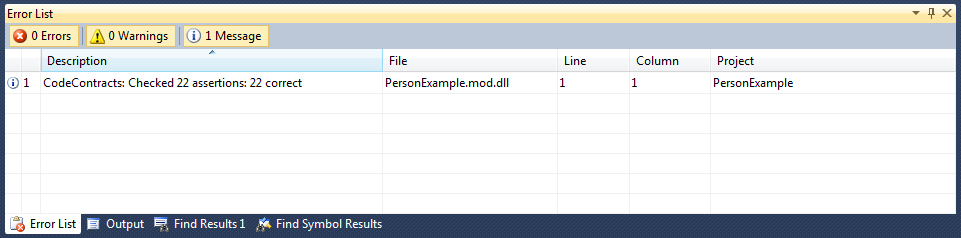
\includegraphics[scale=0.5]{vs_verif_ok.png}
			\end{center}
			\caption{Resultado de verificación correcta}
			\end{figure}

			Mientras que si falló la verificación de algún contrato se verá una salida como la siguiente:

			\begin{figure}[htb]
			\begin{center}
			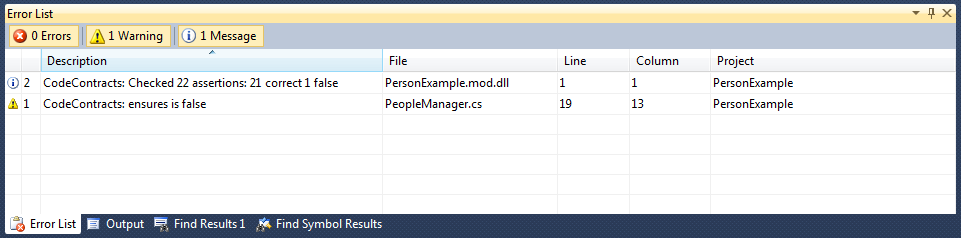
\includegraphics[scale=0.5]{vs_verif_err.png}
			\end{center}
			\caption{Resultado de verificación con contratos no verificados}
			\end{figure}

		\newpage
		\subsection{Ejemplo completo anotado} \label{sec:ejcompanot}
			En esta sección presentamos un conjunto de clases que están completamente anotadas con contratos de memoria que se pueden verificar correctamente con la herramienta desarrollada. Las cuatro clases forman parte de una misma biblioteca de código cuyo objetivo es modelar personas con sus direcciones físicas.

			\vspace{15pt}
			\begin{footnotesize}
			\begin{lstlisting}[caption=Clase Address]
public class Address
{
	public string Street { get; private set; }
	public string City { get; private set; }
	public string State { get; private set; }
	
	public Address(string street, string city, string state)
	{
		Contract.Memory.Tmp<AddressValidator>(1);

		Contract.Memory.DestTmp();
		AddressValidator validator = new AddressValidator();

		if (!validator.IsAddressValid(street, city, state))
		{
			throw new Exception("Address is invalid.");
		}

		this.Street = street;
		this.City = city;
		this.State = state;
	}
}
			\end{lstlisting}
			\end{footnotesize}

			\begin{footnotesize}
			\begin{lstlisting}[caption=Clase AddressValidator]
public class AddressValidator
{
	public bool IsAddressValid(string street, string city, string state)
	{
		return !(String.IsNullOrEmpty(street) ||
					String.IsNullOrEmpty(city) ||
					String.IsNullOrEmpty(state));
	}
}
			\end{lstlisting}
			\end{footnotesize}

			\begin{footnotesize}
			\begin{lstlisting}[caption=Clase Person]
public class Person
{
	public string FirtName { get; private set; }
	public string LastName { get; private set; }
	public Address Address { get; private set; }

	public void MoveTo(string street, string city, string state)
	{
		Contract.Memory.Rsd<Address>(Contract.Memory.This, 1);
		Contract.Memory.Tmp<AddressValidator>(1);

		Contract.Memory.DestRsd(Contract.Memory.This);
		this.Address = new Address(street, city, state);
	}

	public Person(string firstName, string lastName, string street, string city, string state)
	{
		Contract.Memory.Rsd<Address>(Contract.Memory.This, 1);
		Contract.Memory.Tmp<AddressValidator>(1);

		this.FirtName = firstName;
		this.LastName = lastName;

		Contract.Memory.AddRsd(Contract.Memory.This, Contract.Memory.This);
		this.MoveTo(street, city, state);
	}
}
			\end{lstlisting}
			\end{footnotesize}

			\begin{footnotesize}
			\begin{lstlisting}[caption=Clase PeopleManager]
public class PeopleManager
{
	public static Person CreatePerson(string firstName, string lastName, string street, string city, string state)
	{
		Contract.Memory.Rsd<Person>(Contract.Memory.Return, 1);
		Contract.Memory.Rsd<Address>(Contract.Memory.Return, 1);
		Contract.Memory.Tmp<AddressValidator>(1);

		Contract.Memory.AddRsd(Contract.Memory.Return, Contract.Memory.This);
		Contract.Memory.DestRsd(Contract.Memory.Return);
		Person person = new Person(firstName, lastName, street, city, state);

		return person;
	}

	public static Contract.Memory.RsdType rsd_MovePersonTo_person;

	public static void MovePersonTo(Person person, string street, string city, string state)
	{
		Contract.Memory.BindRsd(rsd_MovePersonTo_person, person);
		Contract.Memory.Rsd<Address>(rsd_MovePersonTo_person, 1);
		Contract.Memory.Tmp<AddressValidator>(1);

		Contract.Memory.AddRsd(rsd_MovePersonTo_person, Contract.Memory.This);
		person.MoveTo(street, city, state);
	}

	public static Person[] CreateFamily(List<string> firstNames, string lastName, string street, string city, string state)
	{
		System.Diagnostics.Contracts.Contract.Requires(firstNames.Count > 0);

		Contract.Memory.Rsd<Person>(Contract.Memory.Return, firstNames.Count);
		Contract.Memory.Rsd<Person[]>(Contract.Memory.Return, 1);
		Contract.Memory.Rsd<Address>(Contract.Memory.Return, firstNames.Count);
		Contract.Memory.Tmp<AddressValidator>(1);

		Contract.Memory.DestRsd(Contract.Memory.Return);
		Person[] family = new Person[firstNames.Count];

		for (int i = 0; i < firstNames.Count; i++)
		{
			Contract.Memory.AddRsd(Contract.Memory.Return, Contract.Memory.This);
			Contract.Memory.DestRsd(Contract.Memory.Return);
			Person p = new Person(firstNames[i], lastName, street, city, state);
			family[i] = p;
		}

		return family;
	}

	/// <summary>
	/// Creates a family with the combination of all first and last names
	/// </summary>
	public static Person[] CreateCombinedFamily(List<string> firstNames, List<string> lastNames, string street, string city, string state)
	{
			System.Diagnostics.Contracts.Contract.Requires(firstNames.Count > 0);
			System.Diagnostics.Contracts.Contract.Requires(firstNames.Count == lastNames.Count);

			Contract.Memory.Rsd<Person>(Contract.Memory.Return, firstNames.Count * lastNames.Count);
			Contract.Memory.Rsd<Person[]>(Contract.Memory.Return, 1);
			Contract.Memory.Rsd<Address>(Contract.Memory.Return, firstNames.Count * lastNames.Count);
			Contract.Memory.Tmp<AddressValidator>(1);

			Contract.Memory.DestRsd(Contract.Memory.Return);
			Person[] family = new Person[firstNames.Count * lastNames.Count];

			for (int i = 0; i < firstNames.Count; i++)
			{
				Contract.Memory.IterationSpace(0 <= i && i < firstNames.Count);
				for (int j = 0; j < lastNames.Count; j++)
				{
					Contract.Memory.IterationSpace(0 <= j && j < lastNames.Count);
					Contract.Memory.AddRsd(Contract.Memory.Return, Contract.Memory.This);
					Contract.Memory.DestRsd(Contract.Memory.Return);
					Person p = new Person(firstNames[i], lastNames[j], street, city, state);
					family[i * firstNames.Count + j] = p;
				}
			}

			return family;
	}
}
			\end{lstlisting}
			\end{footnotesize}

		\subsection{Información obtenida del análisis de points-to y escape} \label{sec:infopointsto}
			Del análisis de points-to y escape obtenemos un XML que resume la información de todos los métodos de todas las clases del assembly analizado. El XML devuelto tiene la siguiente estructura:

			\vspace{15pt}
			\begin{footnotesize}
			\begin{lstlisting}[caption=Ejemplo de XML del análisis de points-to y escape]
<ptg>
	<method type="class" name="method1">
		<escape> <!-- nodos que escapan -->
			<node name="node1" />
			<node name="node2" />
		</escape>
		<expressions>
			<expr val="expr1">
				<reaches> <!-- nodos alcanzables por expr1 -->
					<node name="node1">
						<expr val="." /> <!-- node1 es alcanzado expr1 misma -->
					</node>
				</reaches>
			</expr>
			<expr val="expr2">
				<reaches>
					<node name="node1">
						<expr val="f" /> <!-- node1 es alcanzado por expr2.f -->
					</node>
					<node name="node2">
						<expr val="." />
						<expr val="f" /> <!-- node2 es alcanzado por expr y por expr2.f -->
					</node>
				</reaches>
			</expr>
		</expressions>
	</method>
	<method type="class" name="method2">
		...
	</method>
</ptg>
			\end{lstlisting}
			\end{footnotesize}

			El XML especifica para cada método cuáles son los nodos que escapan del mismo (un nodo representa una instancia en memoria o conjunto de instancias en algunos casos) y además especifica las expresiones que alcanzan a cada nodo. En los comentarios se pueden observar ejemplos del tipo de información que nos brinda.

	\newpage
	\section{Bibliografía}
	\bibliography{bib}
\end{document}
